\begin{aosachapter}{A Pedometer in the Real World}{s:pedometer}{Dessy Daskalov}

\aosasecti{A Perfect World}\label{a-perfect-world}

Many software engineers reflecting on their training will remember
having the pleasure of living in a very perfect world. We were taught to
solve discrete problems, with defined parameters, in an ideal domain.

Then we were thrown into the real world, with all of its complexities
and challenges. It's messy, which makes it all the more exciting. When
you can solve a real-life problem, with all of its quirks, you can build
software that really helps people.

In this chapter, we'll examine a problem that looks straightforward on
the surface, and gets tangled very quickly when the real world, and real
people, are thrown into the mix.

We'll work together to build a basic pedometer. We'll start by
discussing the theory behind a pedometer and creating a step counting
solution outside of code. Then, we'll implement our solution in code.
Finally, we'll add a web layer to our code so that we have a friendly
interface for a user to work with.

Let's roll up our sleeves, and prepare to untangle a real-world problem.

\aosasecti{Pedometer Theory}\label{pedometer-theory}

The rise of the mobile device brought with it a trend to collect more
and more data on our daily lives. One type of data many people collect
is the number of steps they've taken over a period of time. This data
can be used for health tracking, training for sporting events, or, for
those of us obsessed with collecting and analyzing data, just for kicks.
Steps can be counted using a pedometer, which often uses data from a
hardware accelerometer as input.

\aosasectii{What's an Accelerometer?}\label{whats-an-accelerometer}

An accelerometer is a piece of hardware that measures acceleration in
the $x$, $y$, and $z$ directions. In today's mobile world, many people
carry an accelerometer with them wherever they go, as it's built into
almost all smartphones currently on the market. The $x$, $y$, and $z$
directions are relative to the phone.

An accelerometer returns a \emph{signal} in 3-dimensional space. A
signal is a set of data points recorded over time. Each component of the
signal is a time series representing acceleration in one of the $x$,
$y$, or $z$ directions. Each point in a time series is the acceleration
in that direction at a specific point in time. Acceleration is measured
in units of g-force, or \emph{g}. One \emph{g} is equal to 9.8 $m/s^2$,
the average acceleration due to gravity on Earth.

The diagram below shows an example acceleration signal from an
accelerometer with the three time series.

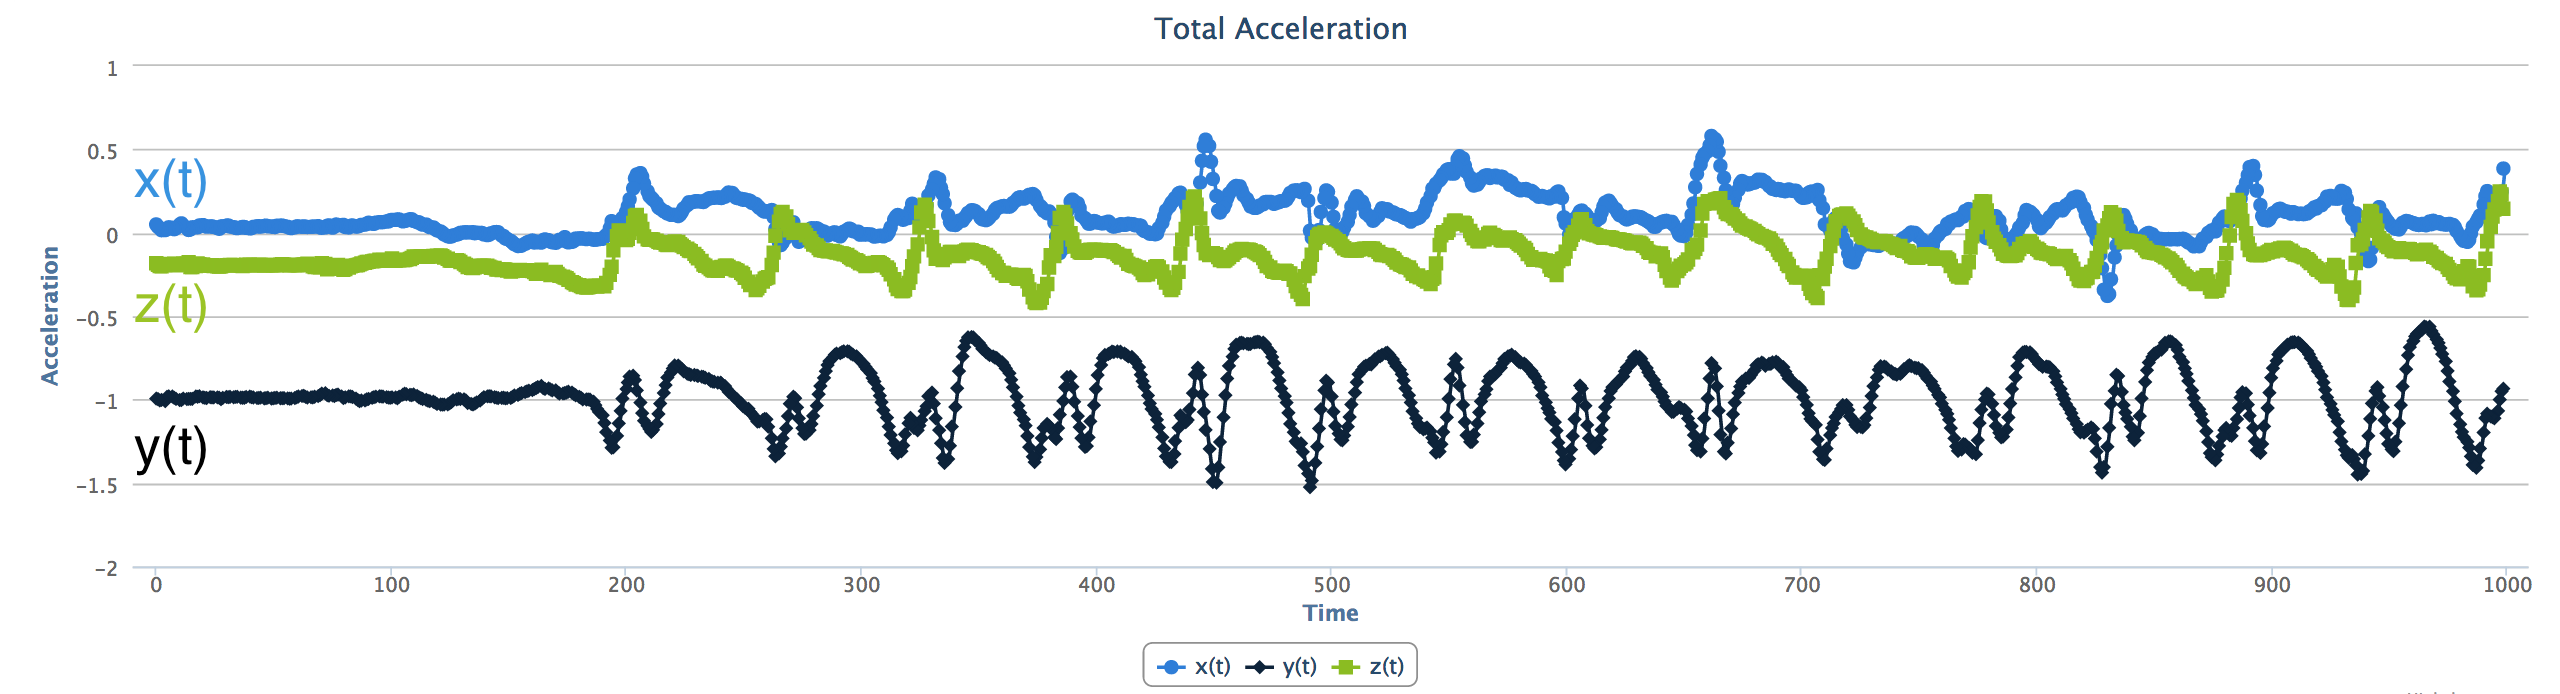
\includegraphics{chapter-figures/acceleration-total.png}\\ The
\emph{sampling rate} of the accelerometer, which can often be
calibrated, determines the number of measurements per second. For
instance, an accelerometer with a sampling rate of 100 returns 100 data
points for each $x$, $y$, and $z$ time series every second.

\aosasectii{Let's Talk About a Walk}\label{lets-talk-about-a-walk}

When a person walks, they bounce slightly with each step. Just watch the
top of a person's head as they walk away from you. Their head, torso,
and hips are synchronized in a smooth bouncing motion. While people
don't bounce very far, only one or two centimeters, it is one of the
clearest, most constant, and most recognizable parts of a person's
walking acceleration signal.

A person bounces up and down, in the vertical direction, with each step.
If you are walking on Earth (or another big ball of mass floating in
space) the bounce is conveniently in the same direction as gravity.

We are going to count steps by using the accelerometer to count bounces
up and down. Because the phone can rotate in any direction, we will take
advantage of gravity to know which direction down is. \textbf{A
pedometer can count steps by counting the number of bounces in the
direction of gravity.}

Let's look at a person walking with an accelerometer-equipped smartphone
in his or her shirt pocket, as depicted below.

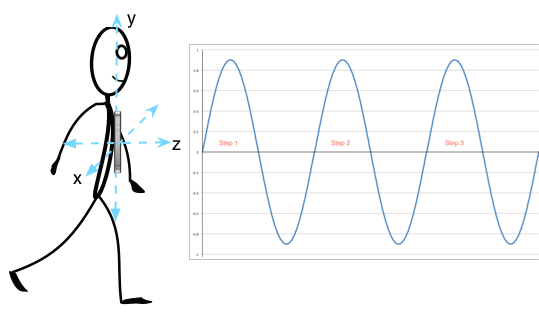
\includegraphics{chapter-figures/walk-1.png}\\ For the sake of
simplicity, we'll assume that the person:

\begin{aosaitemize}

\item
  is walking in the $z$ direction;
\item
  bounces with each step in the $y$ direction; and
\item
  maintains the phone in the same orientation throughout the entire
  walk.
\end{aosaitemize}

In our perfect world, acceleration from step bounces will form a perfect
sine wave in the $y$ direction. Each peak in the sine wave is exactly
one step. Step counting becomes a matter of counting these perfect
peaks.

Ah, the joys of a perfect world, which we only ever experience in texts
like this. Don't fret, things are about to get a little messier, and a
lot more exciting. Let's add a little more reality to our world.

\aosasectii{Even Perfect Worlds Have Fundamental Forces of
Nature}\label{even-perfect-worlds-have-fundamental-forces-of-nature}

The force of gravity causes an acceleration in the direction of gravity,
which we refer to as gravitational acceleration. This acceleration is
unique because it is always present and, for the purposes of this
chapter, is constant at 9.8 $m/s^2$.

Suppose a smartphone is lying on a table screen-side up. In this
orientation, our coordinate system is such that the negative $z$
direction is the one that gravity is acting on. Gravity will pull our
phone in the negative $z$ direction, so our accelerometer, \emph{even
when perfectly still}, will record an acceleration of 9.8 $m/s^2$ in the
negative $z$ direction. Accelerometer data from our phone in this
orientation looks like the graph below.

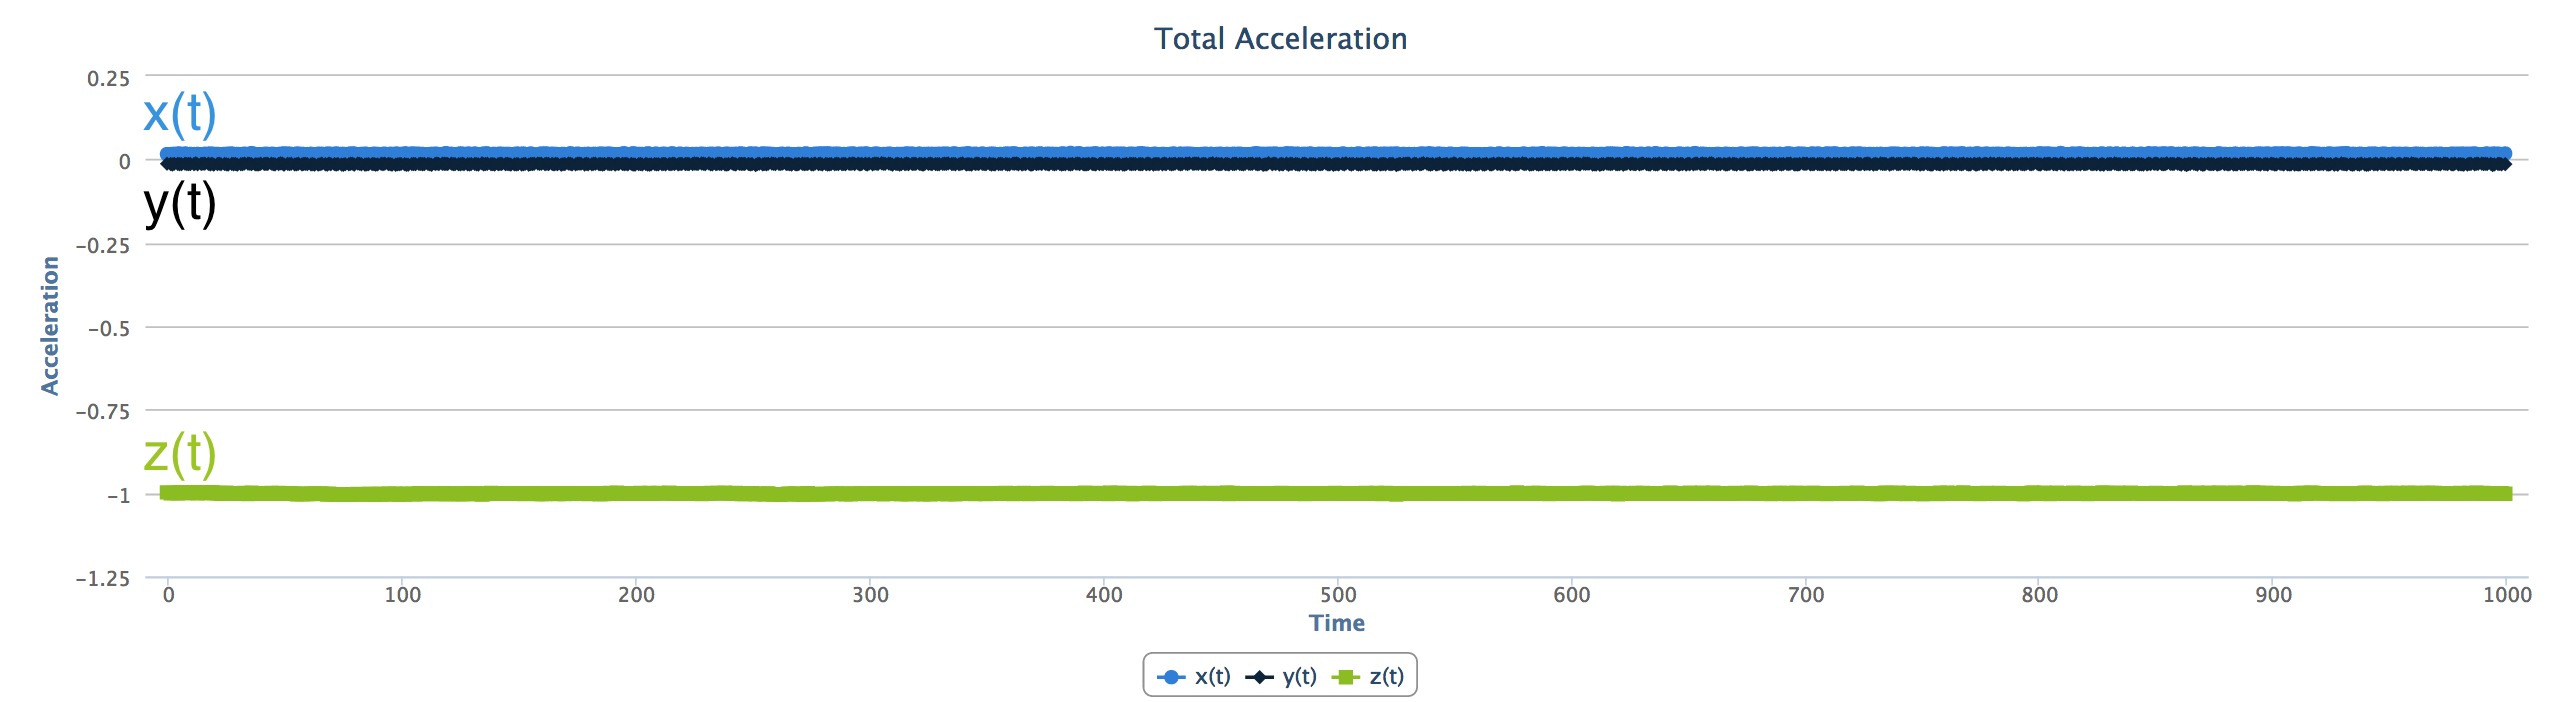
\includegraphics{chapter-figures/acceleration-total-phone-still.png}\\
Note that $x(t)$ and $y(t)$ remain constant at 0, while $z(t)$ is
constant at -1 \emph{g}. Our accelerometer records all acceleration,
including gravitational acceleration.

Each time series measures the \emph{total acceleration} in that
direction. Total acceleration is the sum of \emph{user acceleration} and
\emph{gravitational acceleration}.

User acceleration is the acceleration of the device due to the movement
of the user, and is constant at 0 when the phone is perfectly still.
However, when the user is moving with the device, user acceleration is
rarely constant, since it's difficult for a person to move with a
constant acceleration.

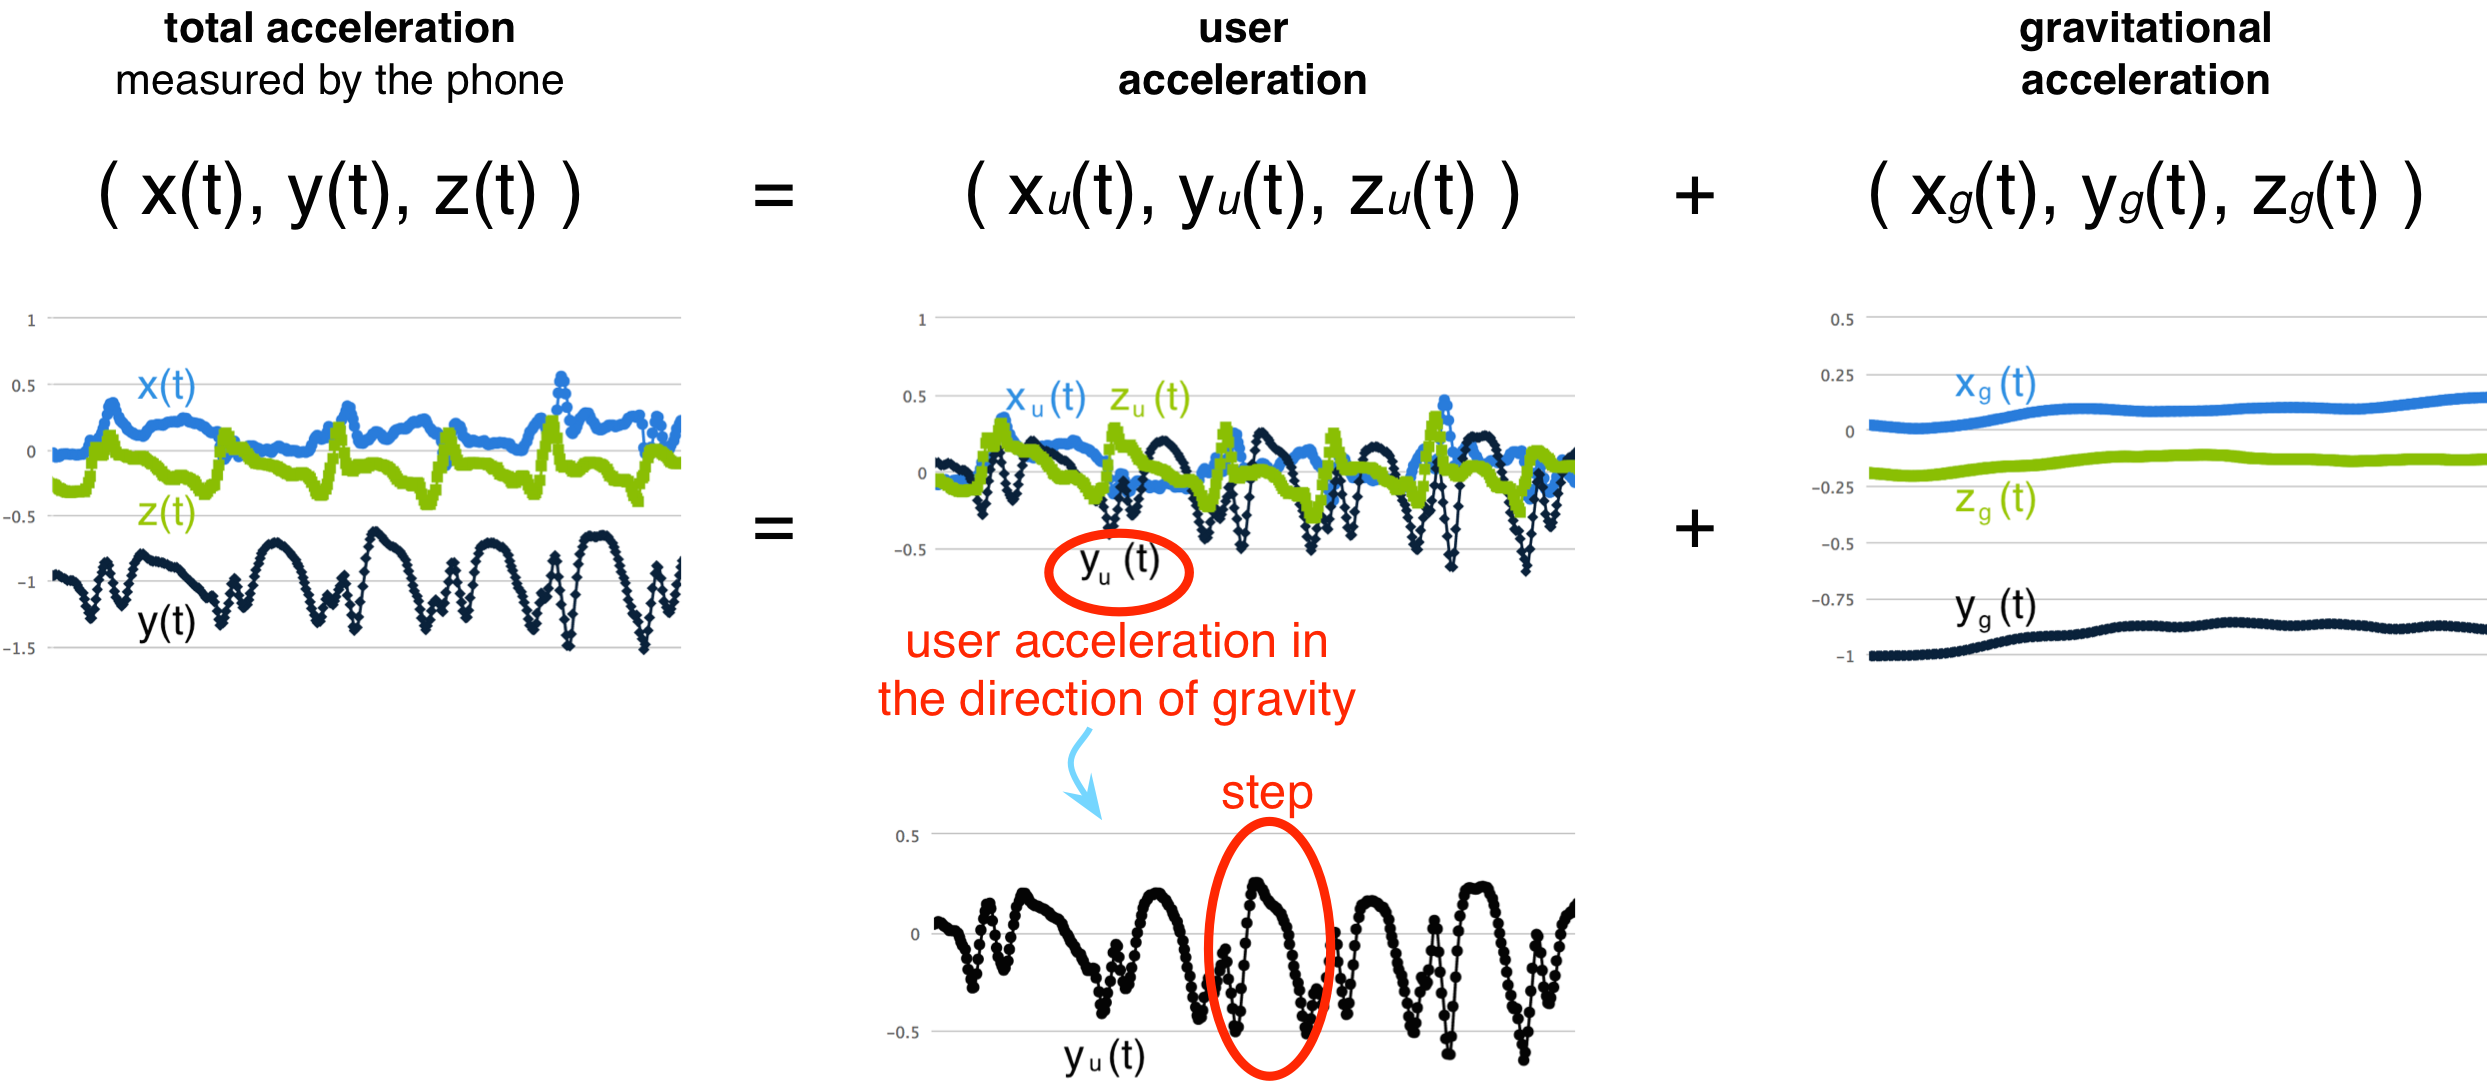
\includegraphics{chapter-figures/component-signals-2.png}\\ To count
steps, we're interested in the bounces created by the user in the
direction of gravity. That means we're interested in isolating the
1-dimensional time series which describes \textbf{user acceleration in
the direction of gravity} from our 3-dimensional acceleration signal.

In our simple example, gravitational acceleration is 0 in $x(t)$ and
$z(t)$ and constant at 9.8 $m/s^2$ in $y(t)$. Therefore, in our total
acceleration plot, $x(t)$ and $z(t)$ fluctuate around 0 while $y(t)$
fluctuates around -1 \emph{g}. In our user acceleration plot, we notice
that --- because we have removed gravitational acceleration --- all
three time series fluctuate around 0. Note the obvious peaks in
$y_{u}(t)$. Those are due to step bounces! In our last plot,
gravitational acceleration, $y_{g}(t)$ is constant at -1 \emph{g}, and
$x_{g}(t)$ and $z_{g}(t)$ are constant at 0.

So, in our example, the 1-dimensional user acceleration in the direction
of gravity time series we're interested in is $y_{u}(t)$. Although
$y_{u}(t)$ isn't as smooth as our perfect sine wave, we can identify the
peaks, and use those peaks to count steps. So far, so good. Now, let's
add even more reality to our world.

\aosasectii{People Are Complicated
Creatures}\label{people-are-complicated-creatures}

What if a person carries the phone in a bag on their shoulder, with the
phone in a more wonky position? To make matters worse, what if the phone
rotates in the bag part way through the walk?

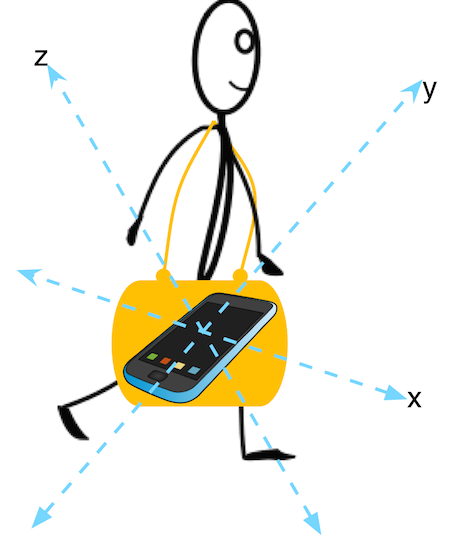
\includegraphics{chapter-figures/walk-2.png}\\ Yikes. Now all three of
our components have a non-zero gravitational acceleration, so the user
acceleration in the direction of gravity is now split amongst all three
time series. To determine user acceleration in the direction of gravity,
we first have to determine which direction gravity is acting in. To do
this, we have to split total acceleration in each of the three time
series into a user acceleration time series and a gravitational
acceleration time series.

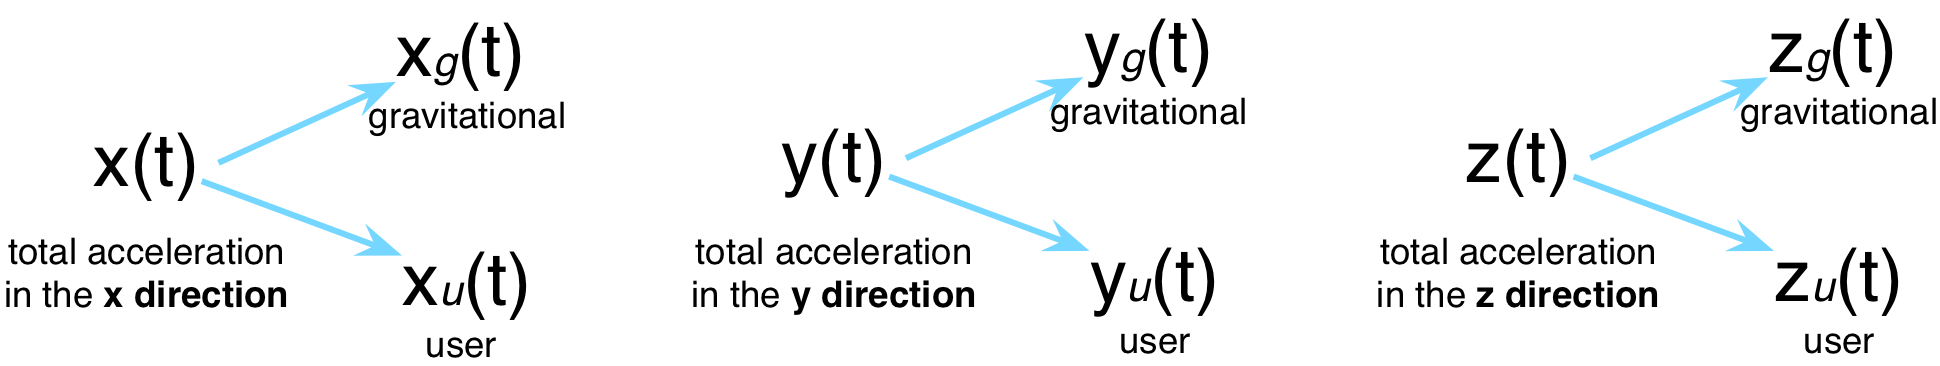
\includegraphics{chapter-figures/component-signals-3.png}\\ Then we can
isolate the portion of user acceleration in each component that is in
the direction of gravity, resulting in just the user acceleration in the
direction of gravity time series.

Let's define this as two steps below:

\begin{aosaenumerate}
\def\labelenumi{\arabic{enumi}.}

\item
  Splitting total acceleration into user acceleration and gravitational
  acceleration.
\item
  Isolating user acceleration in the direction of gravity.
\end{aosaenumerate}

We'll look at each step separately, and put on our mathematician hats.

\aosasectii{1. Splitting Total Acceleration Into User Acceleration and
Gravitational
Acceleration}\label{splitting-total-acceleration-into-user-acceleration-and-gravitational-acceleration}

We can use a tool called a \emph{filter} to split a total acceleration
time series into a user acceleration time series and a gravitational
acceleration time series.

\aosasectiii{Low-Pass and High-Pass
Filters}\label{low-pass-and-high-pass-filters}

A filter is a tool used in signal processing to remove an unwanted
component from a signal.

A \emph{low-pass filter} allows low-frequency signals through, while
attenuating signals higher than a set threshold. Conversely, a
\emph{high-pass filter} allows high-frequency signals through, while
attenuating signals below a set threshold. Using music as an analogy, a
low-pass filter can eliminate treble, and a high-pass filter can
eliminate bass.

In our situation, the frequency, measured in Hz, indicates how quickly
the acceleration is changing. A constant acceleration has a frequency of
0 Hz, while a non-constant acceleration has a non-zero frequency. This
means that our constant gravitational acceleration is a 0 Hz signal,
while user acceleration is not.

For each component, we can pass total acceleration through a low-pass
filter, and we'll be left with just the gravitational acceleration time
series. Then we can subtract gravitational acceleration from total
acceleration, and we'll have the user acceleration time series.

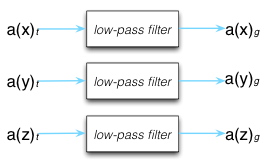
\includegraphics{chapter-figures/low-pass-filter-a.png}\\ There are
numerous varieties of filters. The one we'll use is called an infinite
impulse response (IIR) filter. We've chosen an IIR filter because of its
low overhead and ease of implementation. The IIR filter we've chosen is
implemented using the formula
$output_{i} = \alpha_{0}(input_{i}\beta_{0} + input_{i-1}\beta_{1} + input_{i-2}\beta_{2} - output_{i-1}\alpha_{1} - output_{i-2}\alpha_{2})$.

The design of digital filters is outside of the scope of this chapter,
but a very short teaser discussion is warranted. It's a well-studied,
fascinating topic, with numerous practical applications. A digital
filter can be designed to cancel any frequency or range of frequencies
desired. The $\alpha$ and $\beta$ values in the formula are
coefficients, set based on the cutoff frequency, and the range of
frequencies we want to preserve.

We want to cancel all frequencies except for our constant gravitational
acceleration, so we've chosen coefficients that attenuate frequencies
higher than 0.2 Hz. Notice that we've set our threshold slightly higher
than 0 Hz. While gravity does create a true 0 Hz acceleration, our real,
imperfect world has real, imperfect accelerometers, so we're allowing
for a slight margin of error in measurement.

\aosasectiii{Implementing a Low-Pass
Filter}\label{implementing-a-low-pass-filter}

Let's work through a low-pass filter implementation using our earlier
example. We'll split:

\begin{aosaitemize}

\item
  $x(t)$ into $x_{g}(t)$ and $x_{u}(t)$,
\item
  $y(t)$ into $y_{g}(t)$ and $y_{u}(t)$, and
\item
  $z(t)$ into $z_{g}(t)$ and $z_{u}(t)$.
\end{aosaitemize}

We'll initialize the first two values of gravitational acceleration to
0, so that the formula has initial values to work with.

$x_{g}(0) = x_{g}(1) = y_{g}(0) = y_{g}(1) = z_{g}(0) = z_{g}(1) = 0$

Then we'll implement the filter formula for each time series.

$x_{g}(t) = \alpha_{0}(x(t)\beta_{0} + x(t-1)\beta_{1} + x(t-2)\beta_{2} - x_{g}(t-1)\alpha_{1} - x_{g}(t-2)\alpha_{2})$

$y_{g}(t) = \alpha_{0}(y(t)\beta_{0} + y(t-1)\beta_{1} + y(t-2)\beta_{2} - y_{g}(t-1)\alpha_{1} - y_{g}(t-2)\alpha_{2})$

$z_{g}(t) = \alpha_{0}(z(t)\beta_{0} + z(t-1)\beta_{1} + z(t-2)\beta_{2} - z_{g}(t-1)\alpha_{1} - z_{g}(t-2)\alpha_{2})$

The resulting time series after low-pass filtering are below.

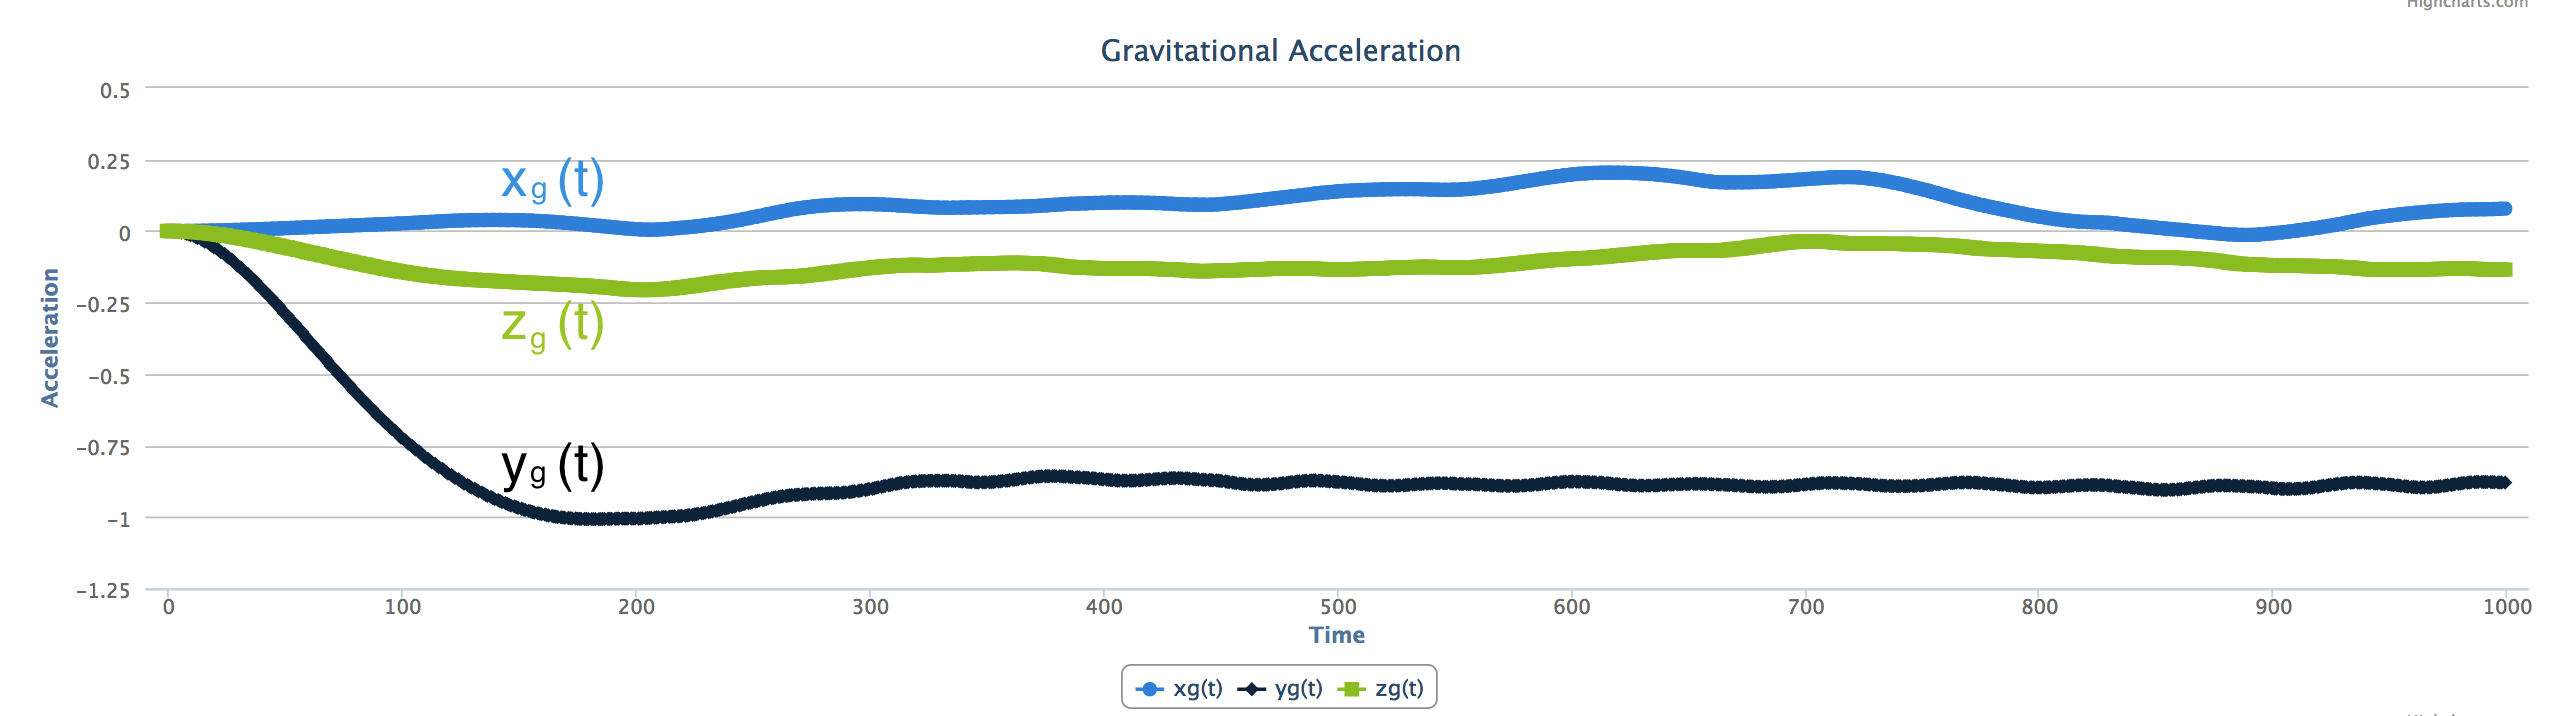
\includegraphics{chapter-figures/acceleration-gravitational.png}\\
$x_{g}(t)$ and $z_{g}(t)$ hover around 0, and $y_{g}(t)$ very quickly
drops to $-1g$. The initial 0 value in $y_{g}(t)$ is from the
initialization of the formula.

Now, to calculate user acceleration, we can subtract gravitational
acceleration from our total acceleration:

\[
x_{u}(t) = x(t) - x_{g}(t)
\] \[
y_{u}(t) = y(t) - y_{g}(t)
\] \[
z_{u}(t) = z(t) - z_{g}(t)
\]

When we do that, we receive the time series below:

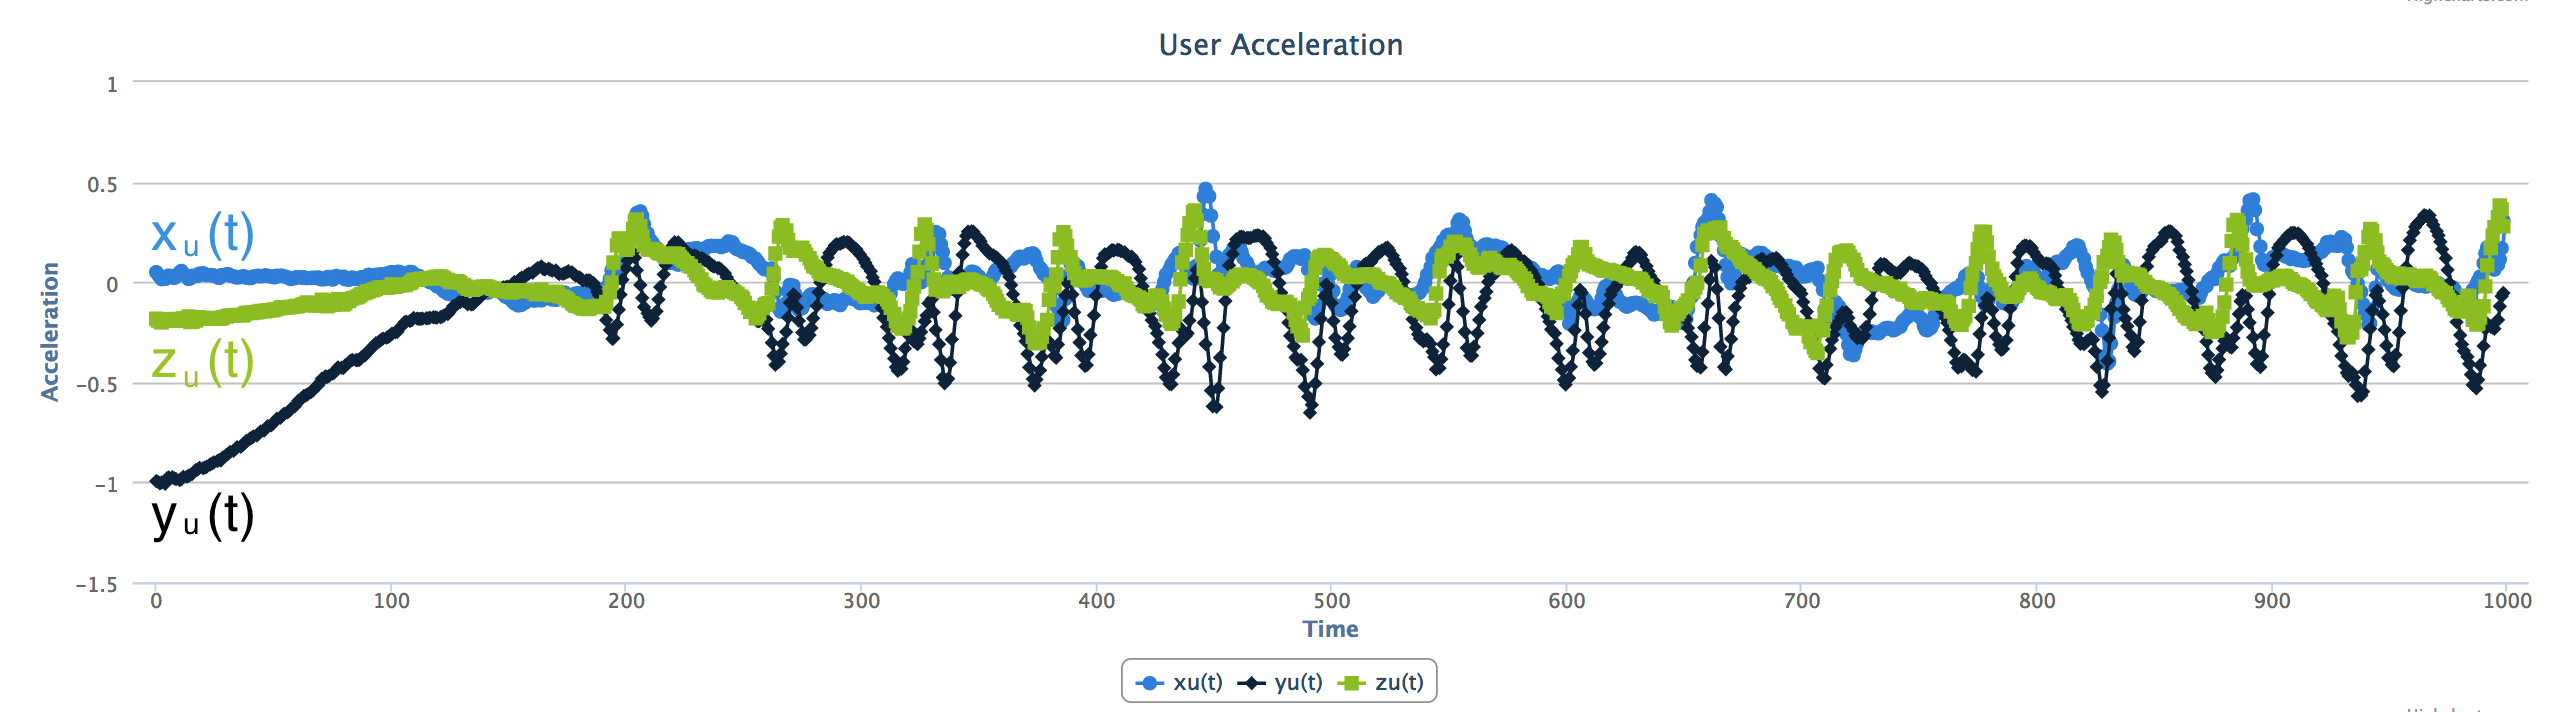
\includegraphics{chapter-figures/acceleration-user.png}\\ We've
successfully split our total acceleration into user acceleration and
gravitational acceleration!

\aosasectii{2. Isolating User Acceleration in the Direction of
Gravity}\label{isolating-user-acceleration-in-the-direction-of-gravity}

$x_{u}(t)$, $y_{u}(t)$, and $z_{u}(t)$ include all movements of the
user, not just movements in the direction of gravity. Our goal here is
to end up with a 1-dimensional time series representing user
acceleration in the direction of gravity. This time series will include
portions of user acceleration in each of the directions.

Let's get to it. First, some linear algebra 101. Don't take that
mathematician hat off just yet!

\aosasectiii{The Dot Product}\label{the-dot-product}

When working with coordinates, you won't get very far before being
introduced to the \emph{dot product}, one of the fundamental tools used
in comparing the magnitude and direction of $x$, $y$, and $z$
coordinates.

The dot product will take us from 3-dimensional space to 1-dimensional
space. When we take the dot product of the two time series, user
acceleration and gravitational acceleration, both of which are in
3-dimensional space, we'll be left with a single time series in
1-dimensional space representing the portion of user acceleration in the
direction of gravity. We'll arbitrarily call this new time series
$a(t)$, because, well, every important time series deserves a name.

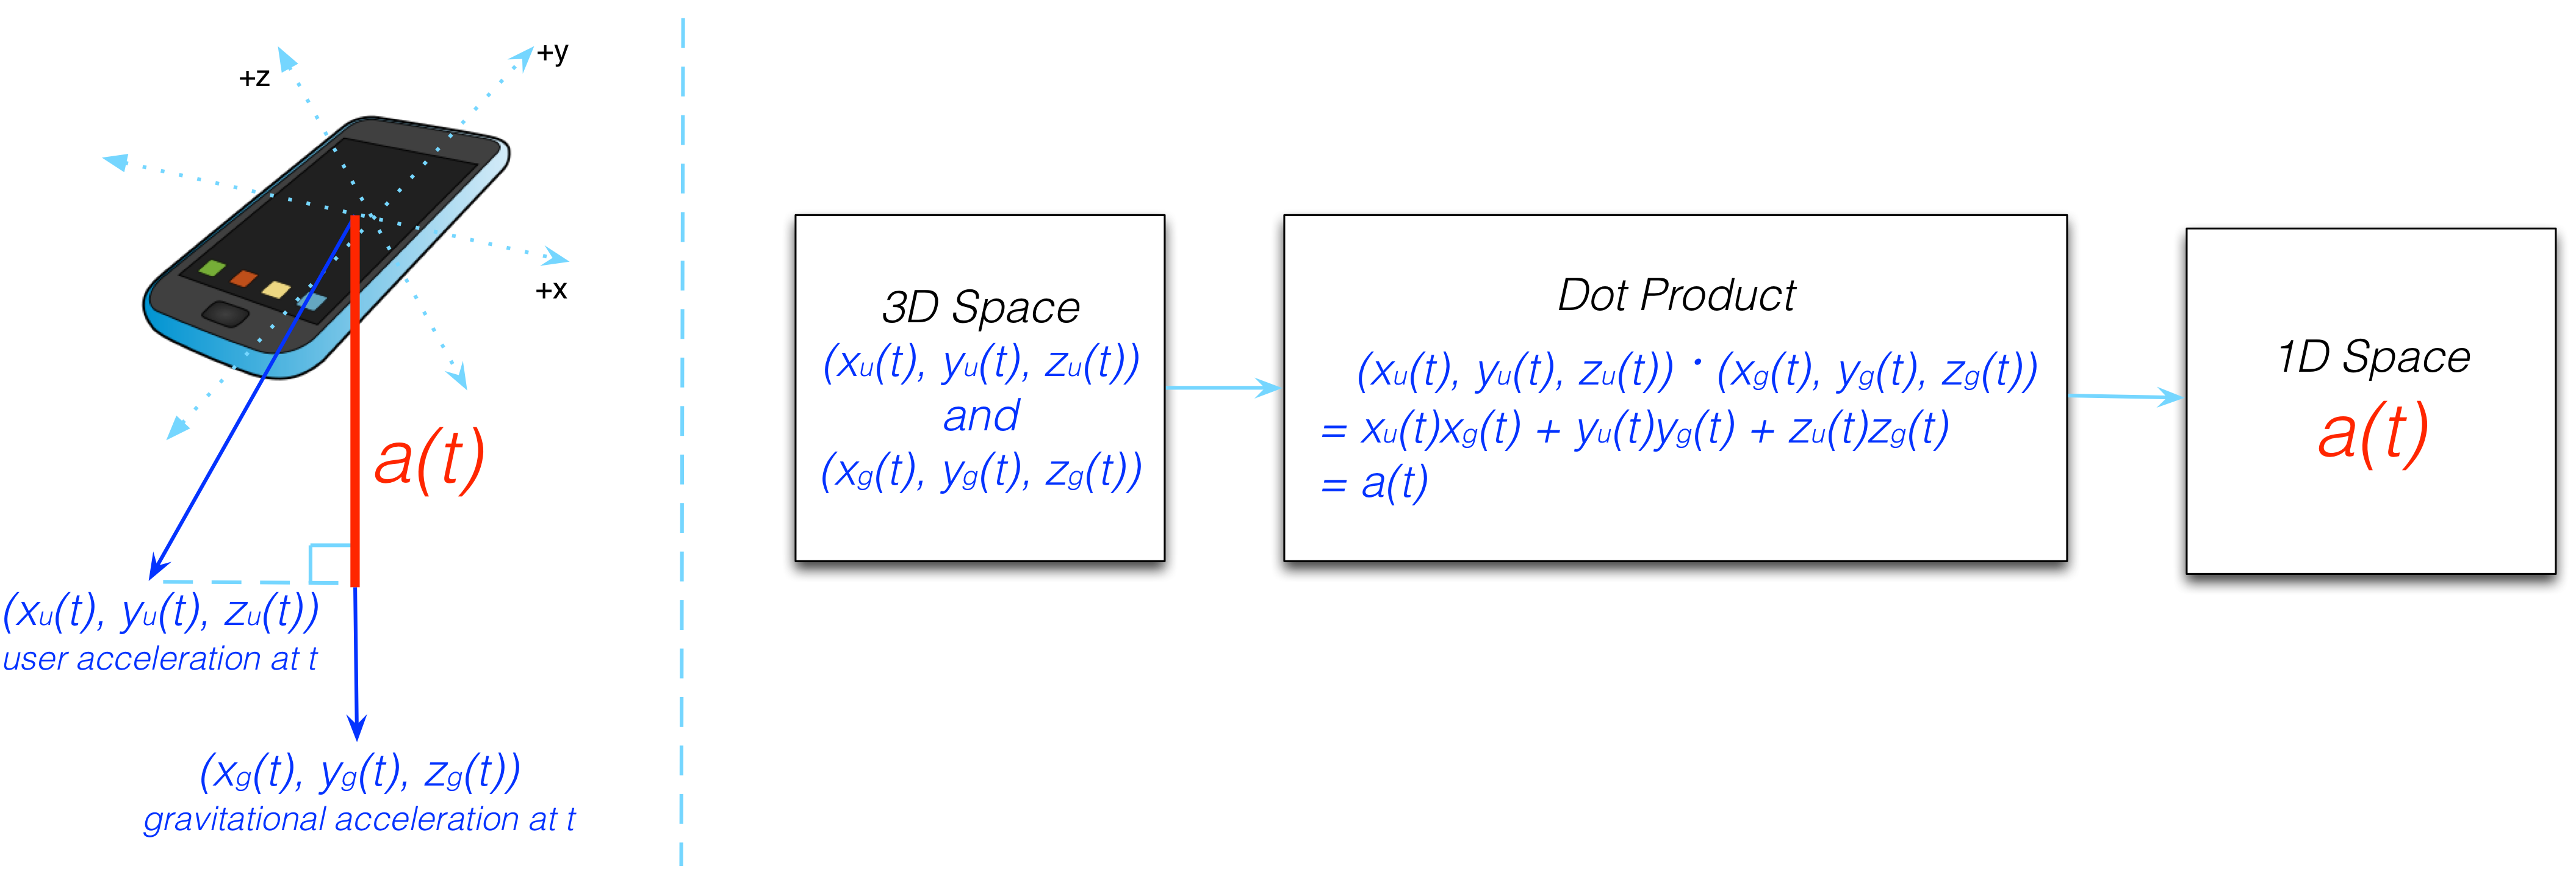
\includegraphics{chapter-figures/dot-product-explanation.png}\\

\aosasectiii{Implementing the Dot
Product}\label{implementing-the-dot-product}

We can implement the dot product for our earlier example using the
formula $a(t) = x_{u}(t)x_{g}(t) + y_{u}(t)y_{g}(t) + z_{u}(t)z_{g}(t)$,
leaving us with $a(t)$ in 1-dimensional space.

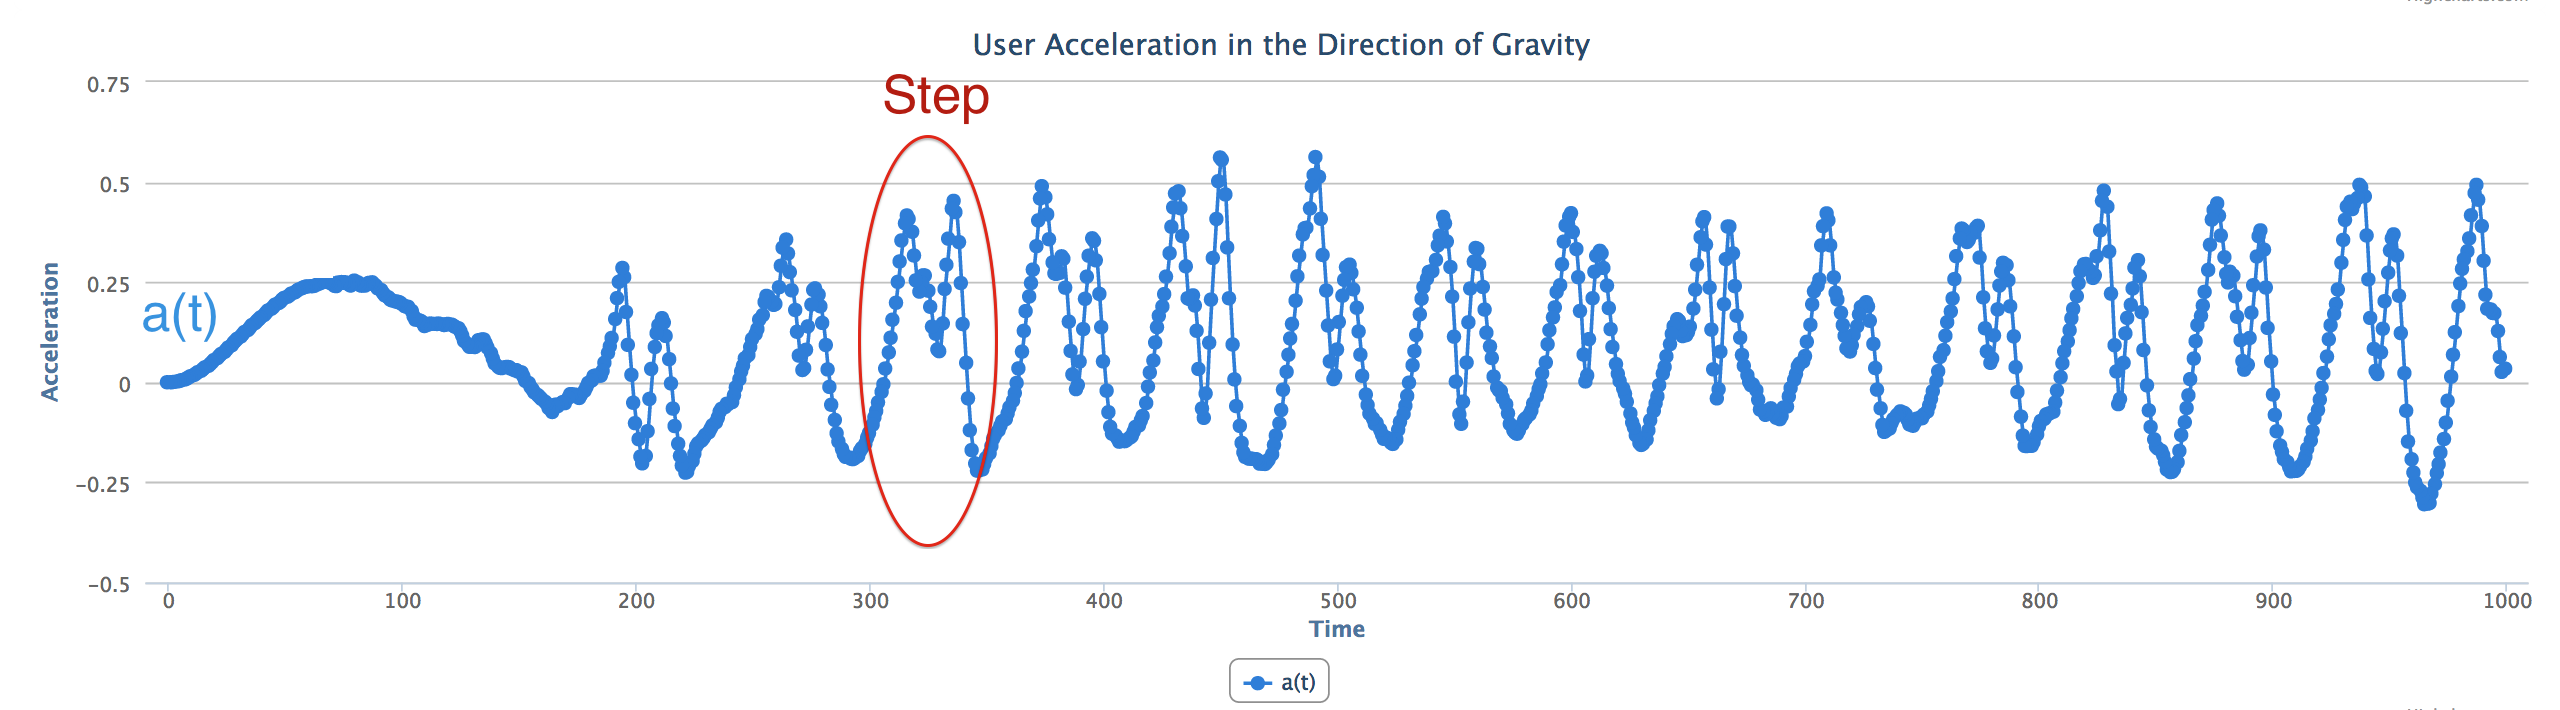
\includegraphics{chapter-figures/acceleration-dotproduct.png}\\ We can
now visually pick out where the steps are in $a(t)$. The dot product is
very powerful, yet beautifully simple.

\aosasectii{Solutions in the Real
World}\label{solutions-in-the-real-world}

We saw how quickly our seemingly simple problem became more complex when
we threw in the challenges of the real world and real people. However,
we're getting a lot closer to counting steps, and we can see how $a(t)$
is starting to resemble our ideal sine wave. But, only ``kinda, sorta''
starting to. We still need to make our messy $a(t)$ time series
smoother. There are four main issues with $a(t)$ in its current state.
Let's examine each one.

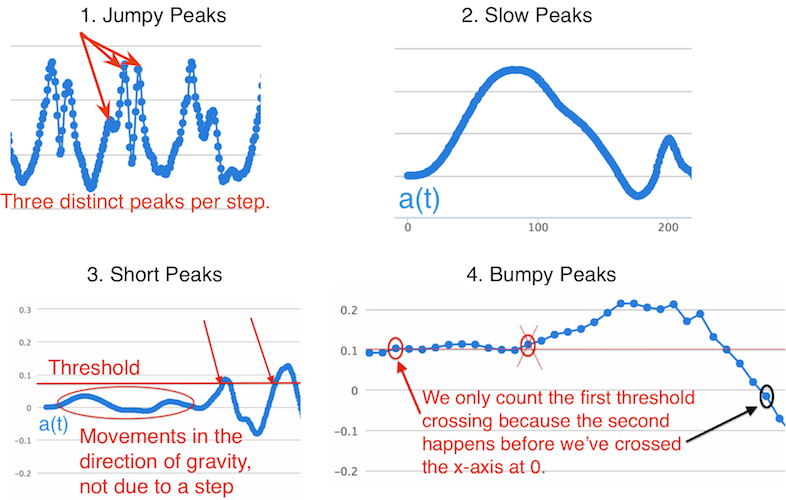
\includegraphics{chapter-figures/jumpy-slow-short-bumpy.png}\\

\aosasectiii{1. Jumpy Peaks}\label{jumpy-peaks}

$a(t)$ is very ``jumpy'', because a phone can jiggle with each step,
adding a high-frequency component to our time series. This jumpiness is
called noise. By studying numerous data sets, we've determined that a
step acceleration is at maximum 5 Hz. We can use a low-pass IIR filter
to remove the noise, picking $\alpha$ and $\beta$ to attenuate all
signals above 5 Hz.

\aosasectiii{2. Slow Peaks}\label{slow-peaks}

With a sampling rate of 100, the slow peak displayed in $a(t)$ spans 1.5
seconds, which is too slow to be a step. In studying enough samples of
data, we've determined that the slowest step we can take is at a 1 Hz
frequency. Slower accelerations are due to a low-frequency component,
that we can again remove using a high-pass IIR filter, setting $\alpha$
and $\beta$ to cancel all signals below 1 Hz.

\aosasectiii{3. Short Peaks}\label{short-peaks}

As a person is using an app or making a call, the accelerometer
registers small movements in the direction of gravity, presenting
themselves as short peaks in our time series. We can eliminate these
short peaks by setting a minimum threshold, and counting a step every
time $a(t)$ crosses that threshold in the positive direction.

\aosasectiii{4. Bumpy Peaks}\label{bumpy-peaks}

Our pedometer should accommodate many people with different walks, so
we've set minimum and maximum step frequencies based on a large sample
size of people and walks. This means that we may sometimes filter
slightly too much or too little. While we'll often have fairly smooth
peaks, we can, once in a while, get a ``bumpier'' peak. The diagram
above zooms in on one such peak.

When bumpiness occurs at our threshold, we can mistakenly count too many
steps for one peak. We'll use a method called \emph{hysteresis} to
address this. Hysteresis refers to the dependence of an output on past
inputs. We can count threshold crossings in the positive direction, as
well as 0 crossings in the negative direction. Then, we only count steps
where a threshold crossing occurs after a 0 crossing, ensuring we count
each step only once.

\aosasectiii{Peaks That Are Juuuust
Right}\label{peaks-that-are-juuuust-right}

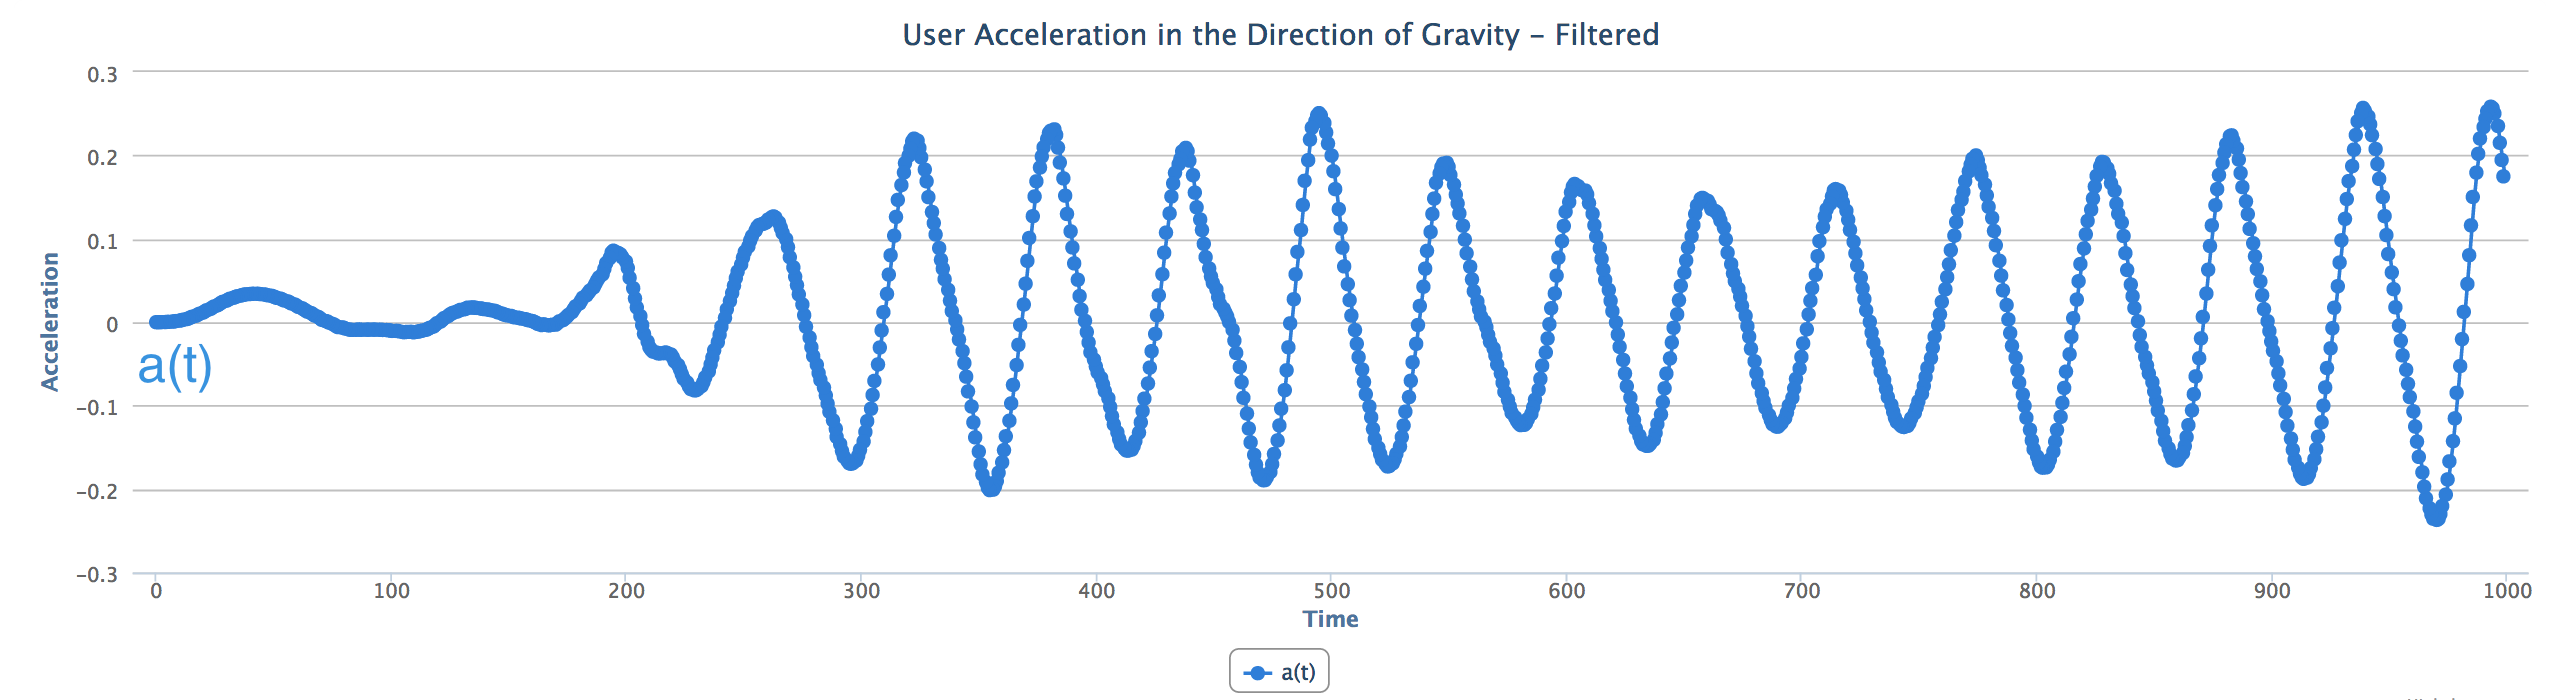
\includegraphics{chapter-figures/acceleration-filtered.png}\\ In
accounting for these four scenarios, we've managed to bring our messy
$a(t)$ fairly close to our ideal sine wave, allowing us to count steps.

\aosasectii{Recap}\label{recap}

The problem, at first glance, looked straightforward. However, the real
world and real people threw a few curve balls our way. Let's recap how
we solved the problem:

\begin{aosaenumerate}
\def\labelenumi{\arabic{enumi}.}

\item
  We started with total acceleration, $(x(t), y(t), z(t))$.
\item
  We used a low-pass filter to split total acceleration into user
  acceleration and gravitational acceleration,
  $(x_{u}(t), y_{u}(t), z_{u}(t))$ and $(x_{g}(t), y_{g}(t), z_{g}(t))$,
  respectively.
\item
  We took the dot product of $(x_{u}(t), y_{u}(t), z_{u}(t))$ and
  $(x_{g}(t), y_{g}(t), z_{g}(t))$ to obtain the user acceleration in
  the direction of gravity, $a(t)$.
\item
  We used a low-pass filter again to remove the high-frequency component
  of $a(t)$, removing noise.
\item
  We used a high-pass filter to cancel the low-frequency component of
  $a(t)$, removing slow peaks.
\item
  We set a threshold to ignore short peaks.
\item
  We used hysteresis to avoid double-counting steps with bumpy peaks.
\end{aosaenumerate}

As software developers in a training or academic setting, we may have
been presented with a perfect signal and asked to write code to count
the steps in that signal. While that may have been an interesting coding
challenge, it wouldn't have been something we could apply in a live
situation. We saw that in reality, with gravity and people thrown into
the mix, the problem was a little more complex. We used mathematical
tools to address the complexities, and were able to solve a real-world
problem. It's time to translate our solution into code.

\aosasecti{Diving Into Code}\label{diving-into-code}

Our goal for this chapter is to create a web application in Ruby that
accepts accelerometer data, parses, processes, and analyzes the data,
and returns the number of steps taken, the distance travelled, and the
elapsed time.

\aosasectii{Preliminary Work}\label{preliminary-work}

Our solution requires us to filter our time series several times. Rather
than peppering filtering code throughout our program, it makes sense to
create a class that takes care of the filtering, and if we ever need to
enhance or modify it, we'll only ever need to change that one class.
This strategy is called \emph{separation of concerns}, a commonly used
design principle which promotes splitting a program into distinct
pieces, where every piece has one primary concern. It's a beautiful way
to write clean, maintainable code that's easily extensible. We'll
revisit this idea several times throughout the chapter.

Let's dive into the filtering code, contained in, logically, a
\texttt{Filter} class.

\begin{verbatim}
class Filter

  COEFFICIENTS_LOW_0_HZ = {
    alpha: [1, -1.979133761292768, 0.979521463540373],
    beta:  [0.000086384997973502, 0.000172769995947004, 0.000086384997973502]
  }
  COEFFICIENTS_LOW_5_HZ = {
    alpha: [1, -1.80898117793047, 0.827224480562408],
    beta:  [0.095465967120306, -0.172688631608676, 0.095465967120306]
  }
  COEFFICIENTS_HIGH_1_HZ = {
    alpha: [1, -1.905384612118461, 0.910092542787947],
    beta:  [0.953986986993339, -1.907503180919730, 0.953986986993339]
  }

  def self.low_0_hz(data)
    filter(data, COEFFICIENTS_LOW_0_HZ)
  end

  def self.low_5_hz(data)
    filter(data, COEFFICIENTS_LOW_5_HZ)
  end

  def self.high_1_hz(data)
    filter(data, COEFFICIENTS_HIGH_1_HZ)
  end

private

  def self.filter(data, coefficients)
    filtered_data = [0,0]
    (2..data.length-1).each do |i|
      filtered_data << coefficients[:alpha][0] *
                      (data[i]            * coefficients[:beta][0] +
                       data[i-1]          * coefficients[:beta][1] +
                       data[i-2]          * coefficients[:beta][2] -
                       filtered_data[i-1] * coefficients[:alpha][1] -
                       filtered_data[i-2] * coefficients[:alpha][2])
    end
    filtered_data
  end

end
\end{verbatim}

Anytime our program needs to filter a time series, we can call one of
the class methods in \texttt{Filter} with the data we need filtered:

\begin{aosaitemize}

\item
  \texttt{low\_0\_hz} is used to low-pass filter signals near 0 Hz
\item
  \texttt{low\_5\_hz} is used to low-pass filter signals at or below 5
  Hz
\item
  \texttt{high\_1\_hz} is used to high-pass filter signals above 1 Hz
\end{aosaitemize}

Each class method calls \texttt{filter}, which implements the IIR filter
and returns the result. If we wish to add more filters in the future, we
only need to change this one class. Note is that all magic numbers are
defined at the top. This makes our class easier to read and understand.

\aosasectii{Input Formats}\label{input-formats}

Our input data is coming from mobile devices such as Android phones and
iPhones. Most mobile phones on the market today have accelerometers
built in, that are able to record total acceleration. Let's call the
input data format that records total acceleration the \emph{combined
format}. Many, but not all, devices can also record user acceleration
and gravitational acceleration separately. Let's call this format the
\emph{separated format}. A device that has the ability to return data in
the separated format necessarily has the ability to return data in the
combined format. However, the inverse is not always true. Some devices
can only record data in the combined format. Input data in the combined
format will need to be passed through a low-pass filter to turn it into
the separated format.

We want our program to handle all mobile devices on the market with
accelerometers, so we'll need to accept data in both formats. Let's look
at the two formats we'll be accepting individually.

\aosasectiii{Combined Format}\label{combined-format}

Data in the combined format is total acceleration in the $x$, $y$, and
$z$ directions, over time. $x$, $y$, and $z$ values will be separated by
a comma, and samples per unit time will be separated by a semi-colon.

\["x1,y1,z1; ... xn,yn,zn;"\]

\aosasectiii{Separated Format}\label{separated-format}

The separated format returns user acceleration and gravitational
acceleration in the $x$, $y$, and $z$ directions, over time. User
acceleration values will be separated from gravitational acceleration
values by a pipe.

\["x^{u}\_1,y^u\_1,z^u\_1|x\^g_1,y^g\_1,z^g\_1; \ldots x^u\_n,y^u\_n,z^u\_n|x^g\_n,y^g\_n,z^g\_n;"\]

\aosasectii{I Got Multiple Input Formats But a Standard Ain't
One}\label{i-got-multiple-input-formats-but-a-standard-aint-one}

Dealing with multiple input formats is a common programming problem. If
we want our entire program to work with both formats, every single piece
of code dealing with the data would need to know how to handle both
formats. This can become very messy, very quickly, especially if a third
(or a fourth, or a fifth, or a hundredth) input format is added.

\aosasectiii{Standard Format}\label{standard-format}

The cleanest way for us to deal with this is to take our two input
formats and fit them into a standard format as soon as possible,
allowing the rest of the program to work with this new standard format.
Our solution requires that we work with user acceleration and
gravitational acceleration separately, so our standard format will need
to be split into the two accelerations:

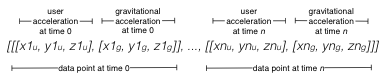
\includegraphics{chapter-figures/standard-format.png}\\ Our standard
format allows us to store a time series, as each element represents
acceleration at a point in time. We've defined it as an array of arrays
of arrays. Let's peel that onion.

\begin{aosaitemize}

\item
  The first array is just a wrapper to hold the all of the data.
\item
  The second set of arrays contains one array per data sample taken. If
  our sampling rate is 100 and we sample data for 10 seconds, we'll have
  $100 * 10$, or 1000, arrays in this second set.
\item
  The third set of arrays is the pair of arrays enclosed within the
  second set. They both contain acceleration data in the $x$, $y$, and
  $z$ directions; the first representing user acceleration and the
  second, gravitational acceleration.
\end{aosaitemize}

\aosasectii{The Pipeline}\label{the-pipeline}

The input into our system will be data from an accelerometer,
information on the user taking the walk (gender, stride, etc.), and
information on the trial walk itself (sampling rate, actual steps taken,
etc.). Our system will apply the signal processing solution, and output
the number of steps calculated, the delta between the actual steps and
calculated steps, the distance travelled, and the elapsed time. The
entire process from input to output can be viewed as a pipeline.

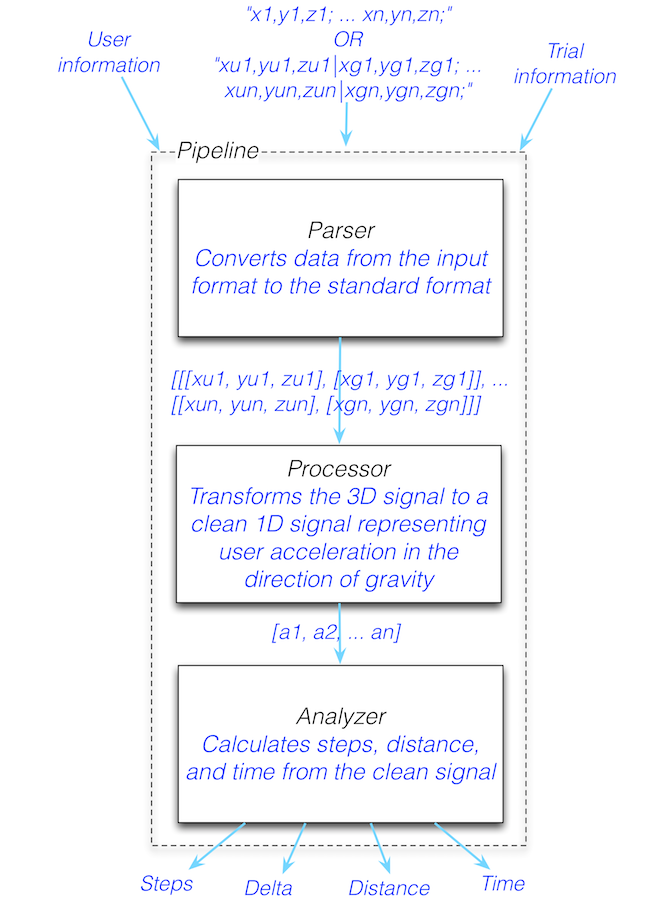
\includegraphics{chapter-figures/pipeline.png}\\ In the spirit of
separation of concerns, we'll write the code for each distinct component
of the pipeline --- parsing, processing, and analyzing --- individually.

\aosasectii{Parsing}\label{parsing}

Given that we want our data in the standard format as early as possible,
it makes sense to write a parser that allows us to take our two known
input formats and convert them to a standard output format as the first
component of our pipeline. Our standard format splits out user
acceleration and gravitational acceleration, which means that if our
data is in the combined format, our parser will need to first pass it
through a low-pass filter to convert it to the standard format.


\includegraphics{chapter-figures/input-data-workflow-1.png}\\ In the
future, if we ever have to add another input format, the only code we'll
have to touch is this parser. Let's separate concerns once more, and
create a \texttt{Parser} class to handle the parsing.

\begin{verbatim}
class Parser

  attr_reader :parsed_data

  def self.run(data)
    parser = Parser.new(data)
    parser.parse
    parser
  end

  def initialize(data)
    @data = data
  end

  def parse
    @parsed_data = @data.to_s.split(';').map { |x| x.split('|') }
                   .map { |x| x.map { |x| x.split(',').map(&:to_f) } }

    unless @parsed_data.map { |x| x.map(&:length).uniq }.uniq == [[3]]
      raise 'Bad Input. Ensure data is properly formatted.'
    end

    if @parsed_data.first.count == 1
      filtered_accl = @parsed_data.map(&:flatten).transpose.map do |total_accl|
        grav = Filter.low_0_hz(total_accl)
        user = total_accl.zip(grav).map { |a, b| a - b }
        [user, grav]
      end

      @parsed_data = @parsed_data.length.times.map do |i|
        user = filtered_accl.map(&:first).map { |elem| elem[i] }
        grav = filtered_accl.map(&:last).map { |elem| elem[i] }
        [user, grav]
      end
    end
  end

end
\end{verbatim}

\texttt{Parser} has a class-level \texttt{run} method as well as an
initializer. This is a pattern we'll use several times, so it's worth a
discussion. Initializers should generally be used for setting up an
object, and shouldn't do a lot of work. \texttt{Parser}'s initializer
simply takes \texttt{data} in the combined or separated format and
stores it in the instance variable \texttt{@data}. The \texttt{parse}
instance method uses \texttt{@data} internally, and does the heavy
lifting of parsing and setting the result in the standard format to
\texttt{@parsed\_data}. In our case, we'll never need to instantiate a
\texttt{Parser} instance without having to immediately call
\texttt{parse}. Therefore, we add a convenient class-level \texttt{run}
method that instantiates an instance of \texttt{Parser}, calls
\texttt{parse} on it, and returns the instance of the object. We can now
pass our input data to \texttt{run}, knowing we'll receive an instance
of \texttt{Parser} with \texttt{@parsed\_data} already set.

Let's take a look at our hard-working \texttt{parse} method. The first
step in the process is to take string data and convert it to numerical
data, giving us an array of arrays of arrays. Sound familiar? The next
thing we do is ensure that the format is as expected. Unless we have
exactly three elements per the innermost arrays, we throw an exception.
Otherwise, we continue on.

Note the differences in \texttt{@parsed\_data} between the two formats
at this stage. In the \emph{combined format} it contains arrays with
exactly \emph{one} array:

\[[[[x1, y1, z1]], ... [[xn, yn, zn]]\]

In the \emph{separated format} it contains arrays with exactly
\emph{two} arrays:

\[[[[x_{u}1,y_{u}1,z_{u}1], [x_{g}1,y_{g}1,z_{g}1]], ... [[x_{u}n,y_{u}n,z_{u}n], [x_{g}n,y_{g}n,z_{g}n]]]\]

The separated format is already in our desired standard format after
this operation. Amazing. However, if the data is combined (or,
equivalently, has exactly one array where the separated format would
have two), then we proceed with two loops. The first loop splits total
acceleration into gravitational and user, using \texttt{Filter} with a
\texttt{:low\_0\_hz} type, and the second loop reorganizes the data into
the standard format.

\texttt{parse} leaves us with \texttt{@parsed\_data} holding data in the
standard format, regardless of whether we started off with combined or
separated data. What a relief!

As our program becomes more sophisticated, one area for improvement is
to make our users' lives easier by throwing exceptions with more
specific error messages, allowing them to more quickly track down common
input formatting problems.

\aosasectii{Processing}\label{processing}

Based on the solution we defined, we'll need our code to do a couple of
things to our parsed data before we can count steps:

\begin{aosaenumerate}
\def\labelenumi{\arabic{enumi}.}

\item
  Isolate movement in the direction of gravity using the dot product.
\item
  Remove jumpy (high-frequency) and slow (low-frequency) peaks with a
  low-pass filter followed by a high-pass filter.
\end{aosaenumerate}

We'll handle short and bumpy peaks by avoiding them during step
counting.

Now that we have our data in the standard format, we can process it to
get in into a state where we can analyze it to count steps.

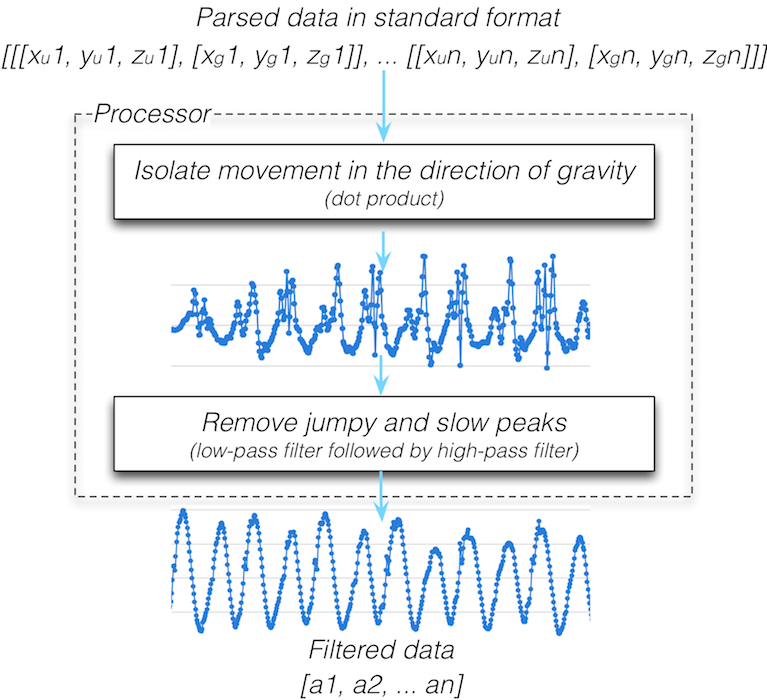
\includegraphics{chapter-figures/input-data-workflow-2.png}\\ The
purpose of processing is to take our data in the standard format and
incrementally clean it up to get it to a state as close as possible to
our ideal sine wave. Our two processing operations, taking the dot
product and filtering, are quite distinct, but both are intended to
process our data, so we'll create one class called a \texttt{Processor}.

\begin{verbatim}
class Processor

  attr_reader :dot_product_data, :filtered_data

  def self.run(data)
    processor = Processor.new(data)
    processor.dot_product
    processor.filter
    processor
  end

  def initialize(data)
    @data = data
  end

  def dot_product
    @dot_product_data = @data.map do |x|
      x[0][0] * x[1][0] + x[0][1] * x[1][1] + x[0][2] * x[1][2]
    end
  end

  def filter
    @filtered_data = Filter.low_5_hz(@dot_product_data)
    @filtered_data = Filter.high_1_hz(@filtered_data)
  end

end
\end{verbatim}

Again, we see the \texttt{run} and \texttt{initialize} methods pattern.
\texttt{run} calls our two processor methods, \texttt{dot\_product} and
\texttt{filter}, directly. Each method accomplishes one of our two
processing operations. \texttt{dot\_product} isolates movement in the
direction of gravity, and \texttt{filter} applies the low-pass and
high-pass filters in sequence to remove jumpy and slow peaks.

\aosasectii{Pedometer Functionality}\label{pedometer-functionality}

Provided information about the person using the pedometer is available,
we can measure more than just steps. Our pedometer will measure
\textbf{distance travelled} and \textbf{elapsed time}, as well as
\textbf{steps taken}.

\aosasectii{Distance Travelled}\label{distance-travelled}

A mobile pedometer is generally used by one person. Distance travelled
during a walk is calculated by multiplying the steps taken by the
person's stride length. If the stride length is unknown, we can use
optional user information like gender and height to approximate it.
Let's create a \texttt{User} class to encapsulate this related
information.

\begin{verbatim}
class User

  GENDER      = ['male', 'female']
  MULTIPLIERS = {'female' => 0.413, 'male' => 0.415}
  AVERAGES    = {'female' => 70.0,  'male' => 78.0}

  attr_reader :gender, :height, :stride

  def initialize(gender = nil, height = nil, stride = nil)
    @gender = gender.to_s.downcase unless gender.to_s.empty?
    @height = Float(height) unless height.to_s.empty?
    @stride = Float(stride) unless stride.to_s.empty?

    raise 'Invalid gender' if @gender && !GENDER.include?(@gender)
    raise 'Invalid height' if @height && (@height <= 0)
    raise 'Invalid stride' if @stride && (@stride <= 0)

    @stride ||= calculate_stride
  end

private

  def calculate_stride
    if gender && height
      MULTIPLIERS[@gender] * height
    elsif height
      height * (MULTIPLIERS.values.reduce(:+) / MULTIPLIERS.size)
    elsif gender
      AVERAGES[gender]
    else
      AVERAGES.values.reduce(:+) / AVERAGES.size
    end
  end

end
\end{verbatim}

At the top of our class, we define constants to avoid hardcoding magic
numbers and strings throughout. For the purposes of this discussion,
let's assume that the values in \texttt{MULTIPLIERS} and
\texttt{AVERAGES} have been determined from a large sample size of
diverse people.

Our initializer accepts \texttt{gender}, \texttt{height}, and
\texttt{stride} as optional arguments. If the optional parameters are
passed in, our initializer sets instance variables of the same names,
after some data formatting. We raise an exception for invalid values.

Even when all optional parameters are provided, the input stride takes
precedence. If it's not provided, the \texttt{calculate\_stride} method
determines the most accurate stride length possible for the user. This
is done with an \texttt{if} statement:

\begin{aosaitemize}

\item
  The most accurate way to calculate stride length is to use a person's
  height and a multiplier based on gender, provided we have a valid
  gender and height.
\item
  A person's height is a better predictor of stride than their gender
  is. If we have height but not gender, we can multiply the height by
  the average of the two values in \texttt{MULTIPLIERS}.
\item
  If all we have is a gender, we can use the average stride length from
  \texttt{AVERAGES}.
\item
  Finally, if we don't have anything, we can take the average of the two
  values in \texttt{AVERAGES} and use that as our stride.
\end{aosaitemize}

Note that the further down the \texttt{if} statement we get, the less
accurate our stride length becomes. In any case, our \texttt{User} class
determines the stride length as best it can.

\aosasectii{Elapsed Time}\label{elapsed-time}

The time spent travelling is measured by dividing the number of data
samples in our \texttt{Processor}'s \texttt{@parsed\_data} by the
sampling rate of the device, if we have it. Since the rate has more to
do with the trial walk itself than the user, and the \texttt{User} class
in fact does not have to be aware of the sampling rate, this is a good
time to create a very small \texttt{Trial} class.

\begin{verbatim}
class Trial

  attr_reader :name, :rate, :steps

  def initialize(name, rate = nil, steps = nil)
    @name  = name.to_s.delete(' ')
    @rate  = Integer(rate.to_s) unless rate.to_s.empty?
    @steps = Integer(steps.to_s) unless steps.to_s.empty?

    raise 'Invalid name'  if @name.empty?
    raise 'Invalid rate'  if @rate && (@rate <= 0)
    raise 'Invalid steps' if @steps && (@steps < 0)
  end

end
\end{verbatim}

All of the attribute readers in \texttt{Trial} are set in the
initializer based on parameters passed in, as follows:

\begin{aosaitemize}

\item
  \texttt{name} is a name for the specific trial, to help differentiate
  between the different trials.
\item
  \texttt{rate} is the sampling rate of the accelerometer during the
  trial.
\item
  \texttt{steps} is used to set the actual steps taken, so that we can
  record the difference between the actual steps the user took and the
  ones our program counted.
\end{aosaitemize}

Much like our \texttt{User} class, some information is optional. We're
given the opportunity to input details of the trial, if we have it. If
we don't have those details, our program bypasses calculating the
additional results, such as time spent travelling. Another similarity to
our \texttt{User} class is the prevention of invalid values.

\aosasectii{Steps Taken}\label{steps-taken}

It's time to implement our step counting strategy in code. So far, we
have a \texttt{Processor} class that contains \texttt{@filtered\_data},
which is our clean time series representing user acceleration in the
direction of gravity. We also have classes that give us the necessary
information about the user and the trial. What we're missing is a way to
analyze \texttt{@filtered\_data} with the information from \texttt{User}
and \texttt{Trial}, and count steps, measure distance, and measure time.

The analysis portion of our program is different from the data
manipulation of the \texttt{Processor}, and different from the
information collection and aggregation of the \texttt{User} and
\texttt{Trial} classes. Let's create a new class called
\texttt{Analyzer} to perform this data analysis.

\begin{verbatim}
class Analyzer

  THRESHOLD = 0.09

  attr_reader :steps, :delta, :distance, :time

  def self.run(data, user, trial)
    analyzer = Analyzer.new(data, user, trial)
    analyzer.measure_steps
    analyzer.measure_delta
    analyzer.measure_distance
    analyzer.measure_time
    analyzer
  end

  def initialize(data, user, trial)
    @data  = data
    @user  = user
    @trial = trial
  end

  def measure_steps
    @steps = 0
    count_steps = true

    @data.each_with_index do |data, i|
      if (data >= THRESHOLD) && (@data[i-1] < THRESHOLD)
        next unless count_steps

        @steps += 1
        count_steps = false
      end

      count_steps = true if (data < 0) && (@data[i-1] >= 0)
    end
  end

  def measure_delta
    @delta = @steps - @trial.steps if @trial.steps
  end

  def measure_distance
    @distance = @user.stride * @steps
  end

  def measure_time
    @time = @data.count/@trial.rate if @trial.rate
  end

end
\end{verbatim}

The first thing we do in \texttt{Analyzer} is define a
\texttt{THRESHOLD} constant, which we'll use to avoid counting short
peaks as steps. For the purposes of this discussion, let's assume we've
analyzed numerous diverse data sets and determined a threshold value
that accommodated the largest number of those data sets. The threshold
can eventually become dynamic and vary with different users, based on
the calculated versus actual steps they've taken; a learning algorithm,
if you will.

Our \texttt{Analyzer}'s initializer takes a \texttt{data} parameter and
instances of \texttt{User} and \texttt{Trial}, and sets the instance
variables \texttt{@data}, \texttt{@user}, and \texttt{@trial} to the
passed-in parameters. The \texttt{run} method calls
\texttt{measure\_steps}, \texttt{measure\_delta},
\texttt{measure\_distance}, and \texttt{measure\_time}. Let's take a
look at each method.

\aosasectiii{\texttt{measure\_steps}}\label{measureux5fsteps}

Finally! The step counting portion of our step counting app. The first
thing we do in \texttt{measure\_steps} is initialize two variables:

\begin{aosaitemize}

\item
  \texttt{@steps} is used to count the number of steps.
\item
  \texttt{count\_steps} is used for hysteresis to determine if we're
  allowed to count steps at a point in time.
\end{aosaitemize}

We then iterate through \texttt{@processor.filtered\_data}. If the
current value is greater than or equal to \texttt{THRESHOLD}, and the
previous value was less than \texttt{THRESHOLD}, then we've crossed the
threshold in the positive direction, which could indicate a step. The
\texttt{unless} statement skips ahead to the next data point if
\texttt{count\_steps} is \texttt{false}, indicating that we've already
counted a step for that peak. If we haven't, we increment
\texttt{@steps} by 1, and set \texttt{count\_steps} to \texttt{false} to
prevent any more steps from being counted for that peak. The next
\texttt{if} statement sets \texttt{count\_steps} to true once our time
series has crossed the $x$-axis in the negative direction, and we're on
to the next peak.

There we have it, the step counting portion of our program! Our
\texttt{Processor} class did a lot of work to clean up the time series
and remove frequencies that would result in counting false steps, so our
actual step counting implementation is not complex.

It's worth noting that we store the entire time series for the walk in
memory. Our trials are all short walks, so that's not currently a
problem, but eventually we'd like to analyze long walks with large
amounts of data. Ideally, we'd want to stream data in, only storing very
small portions of the time series in memory. Keeping this in mind, we've
put in the work to ensure that we only need the current data point and
the data point before it. Additionally, we've implemented hysteresis
using a Boolean value, so we don't need to look backward in the time
series to ensure we've crossed the $x$-axis at 0.

There's a fine balance between accounting for likely future iterations
of the product, and over-engineering a solution for every conceivable
product direction under the sun. In this case, it's reasonable to assume
that we'll have to handle longer walks in the near future, and the costs
of accounting for that in step counting are fairly low.

\aosasectiii{\texttt{measure\_delta}}\label{measureux5fdelta}

If the trial provides actual steps taken during the walk,
\texttt{measure\_delta} will return the difference between the
calculated and actual steps.

\aosasectiii{\texttt{measure\_distance}}\label{measureux5fdistance}

The distance is measured by multiplying our user's stride by the number
of steps. Since the distance depends on the step count,
\texttt{measure\_steps} must be called before
\texttt{measure\_distance}.

\aosasectiii{\texttt{measure\_time}}\label{measureux5ftime}

As long as we have a sampling rate, time is calculated by dividing the
total number of samples in \texttt{filtered\_data} by the sampling rate.
It follows, then, that time is calculated in seconds.

\aosasectii{Tying It All Together With the
Pipeline}\label{tying-it-all-together-with-the-pipeline}

Our \texttt{Parser}, \texttt{Processor}, and \texttt{Analyzer} classes,
while useful individually, are definitely better together. Our program
will often use them to run through the pipeline we introduced earlier.
Since the pipeline will need to be run frequently, we'll create a
\texttt{Pipeline} class to run it for us.

\begin{verbatim}
class Pipeline

  attr_reader :data, :user, :trial, :parser, :processor, :analyzer

  def self.run(data, user, trial)
    pipeline = Pipeline.new(data, user, trial)
    pipeline.feed
    pipeline
  end

  def initialize(data, user, trial)
    @data  = data
    @user  = user
    @trial = trial
  end

  def feed
    @parser    = Parser.run(@data)
    @processor = Processor.run(@parser.parsed_data)
    @analyzer  = Analyzer.run(@processor.filtered_data, @user, @trial)
  end

end
\end{verbatim}

We use our now-familiar \texttt{run} pattern and supply
\texttt{Pipeline} with accelerometer data, and instances of
\texttt{User} and \texttt{Trial}. The \texttt{feed} method implements
the pipeline, which entails running \texttt{Parser} with the
accelerometer data, then using the parser's parsed data to run
\texttt{Processor}, and finally using the processor's filtered data to
run \texttt{Analyzer}. The \texttt{Pipeline} keeps \texttt{@parser},
\texttt{@processor}, and \texttt{@analyzer} instance variables, so that
the program has access to information from those objects for display
purposes through the app.

\aosasecti{Adding A Friendly Interface}\label{adding-a-friendly-interface}

We're through the most labour intensive part of our program. Next, we'll
build a web app to present the data in a format that is pleasing to a
user. A web app naturally separates the data processing from the
presentation of the data. Let's look at our app from a user's
perspective before we dive into the code.

\aosasectii{A User Scenario}\label{a-user-scenario}

When a user first enters the app by navigating to \texttt{/uploads},
they see a table of existing data and a form to submit new data by
uploading an accelerometer output file and trial and user information.

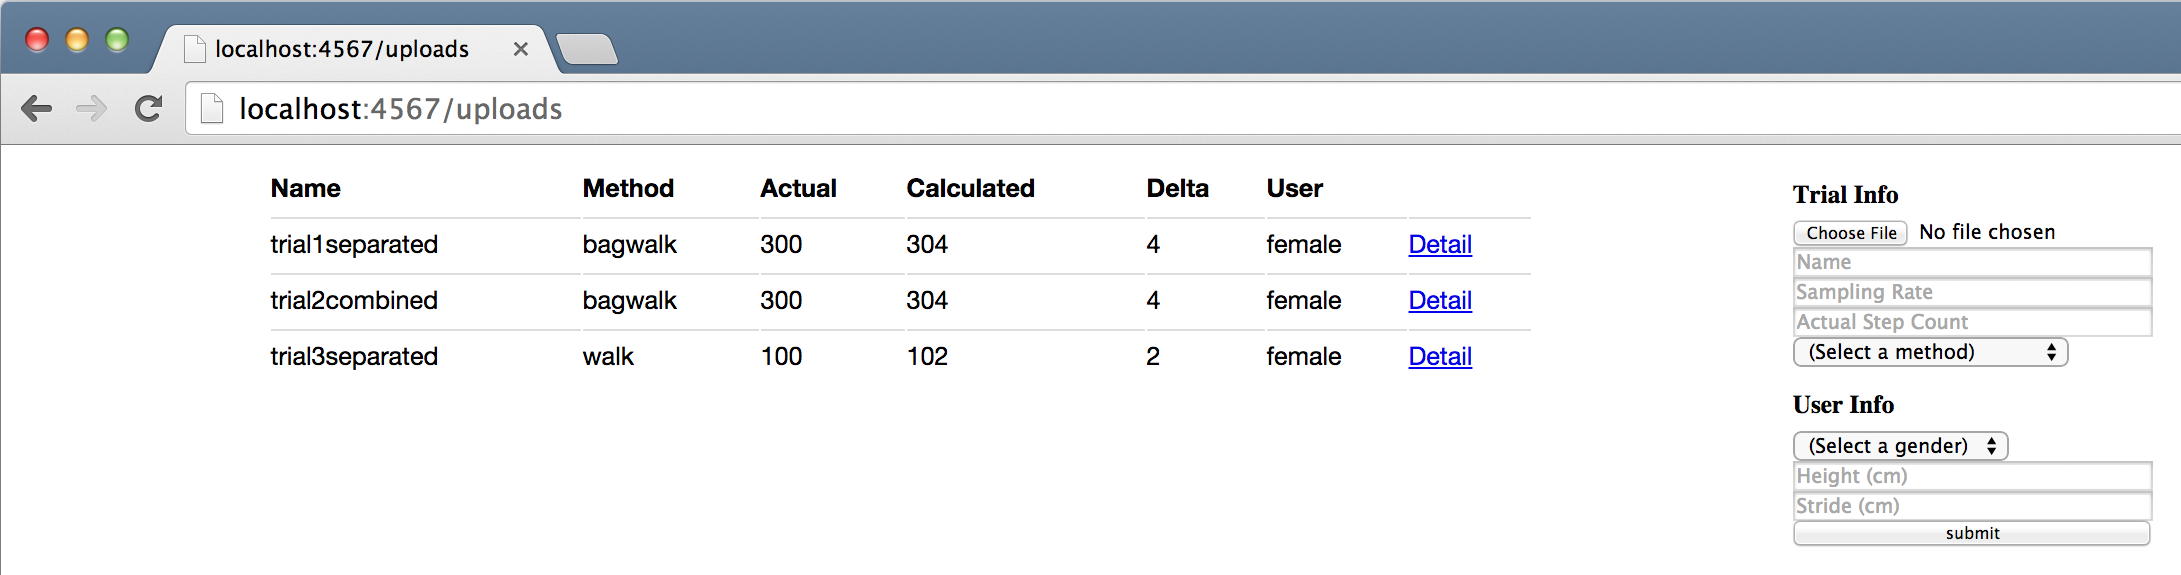
\includegraphics{chapter-figures/graffles/app1.png}\\ Submitting the
form stores the data to the file system, parses, processes, and analyzes
it, and redirects back to \texttt{/uploads} with the new entry in the
table.

Clicking the \textbf{Detail} link for an entry presents the user with
the following view:

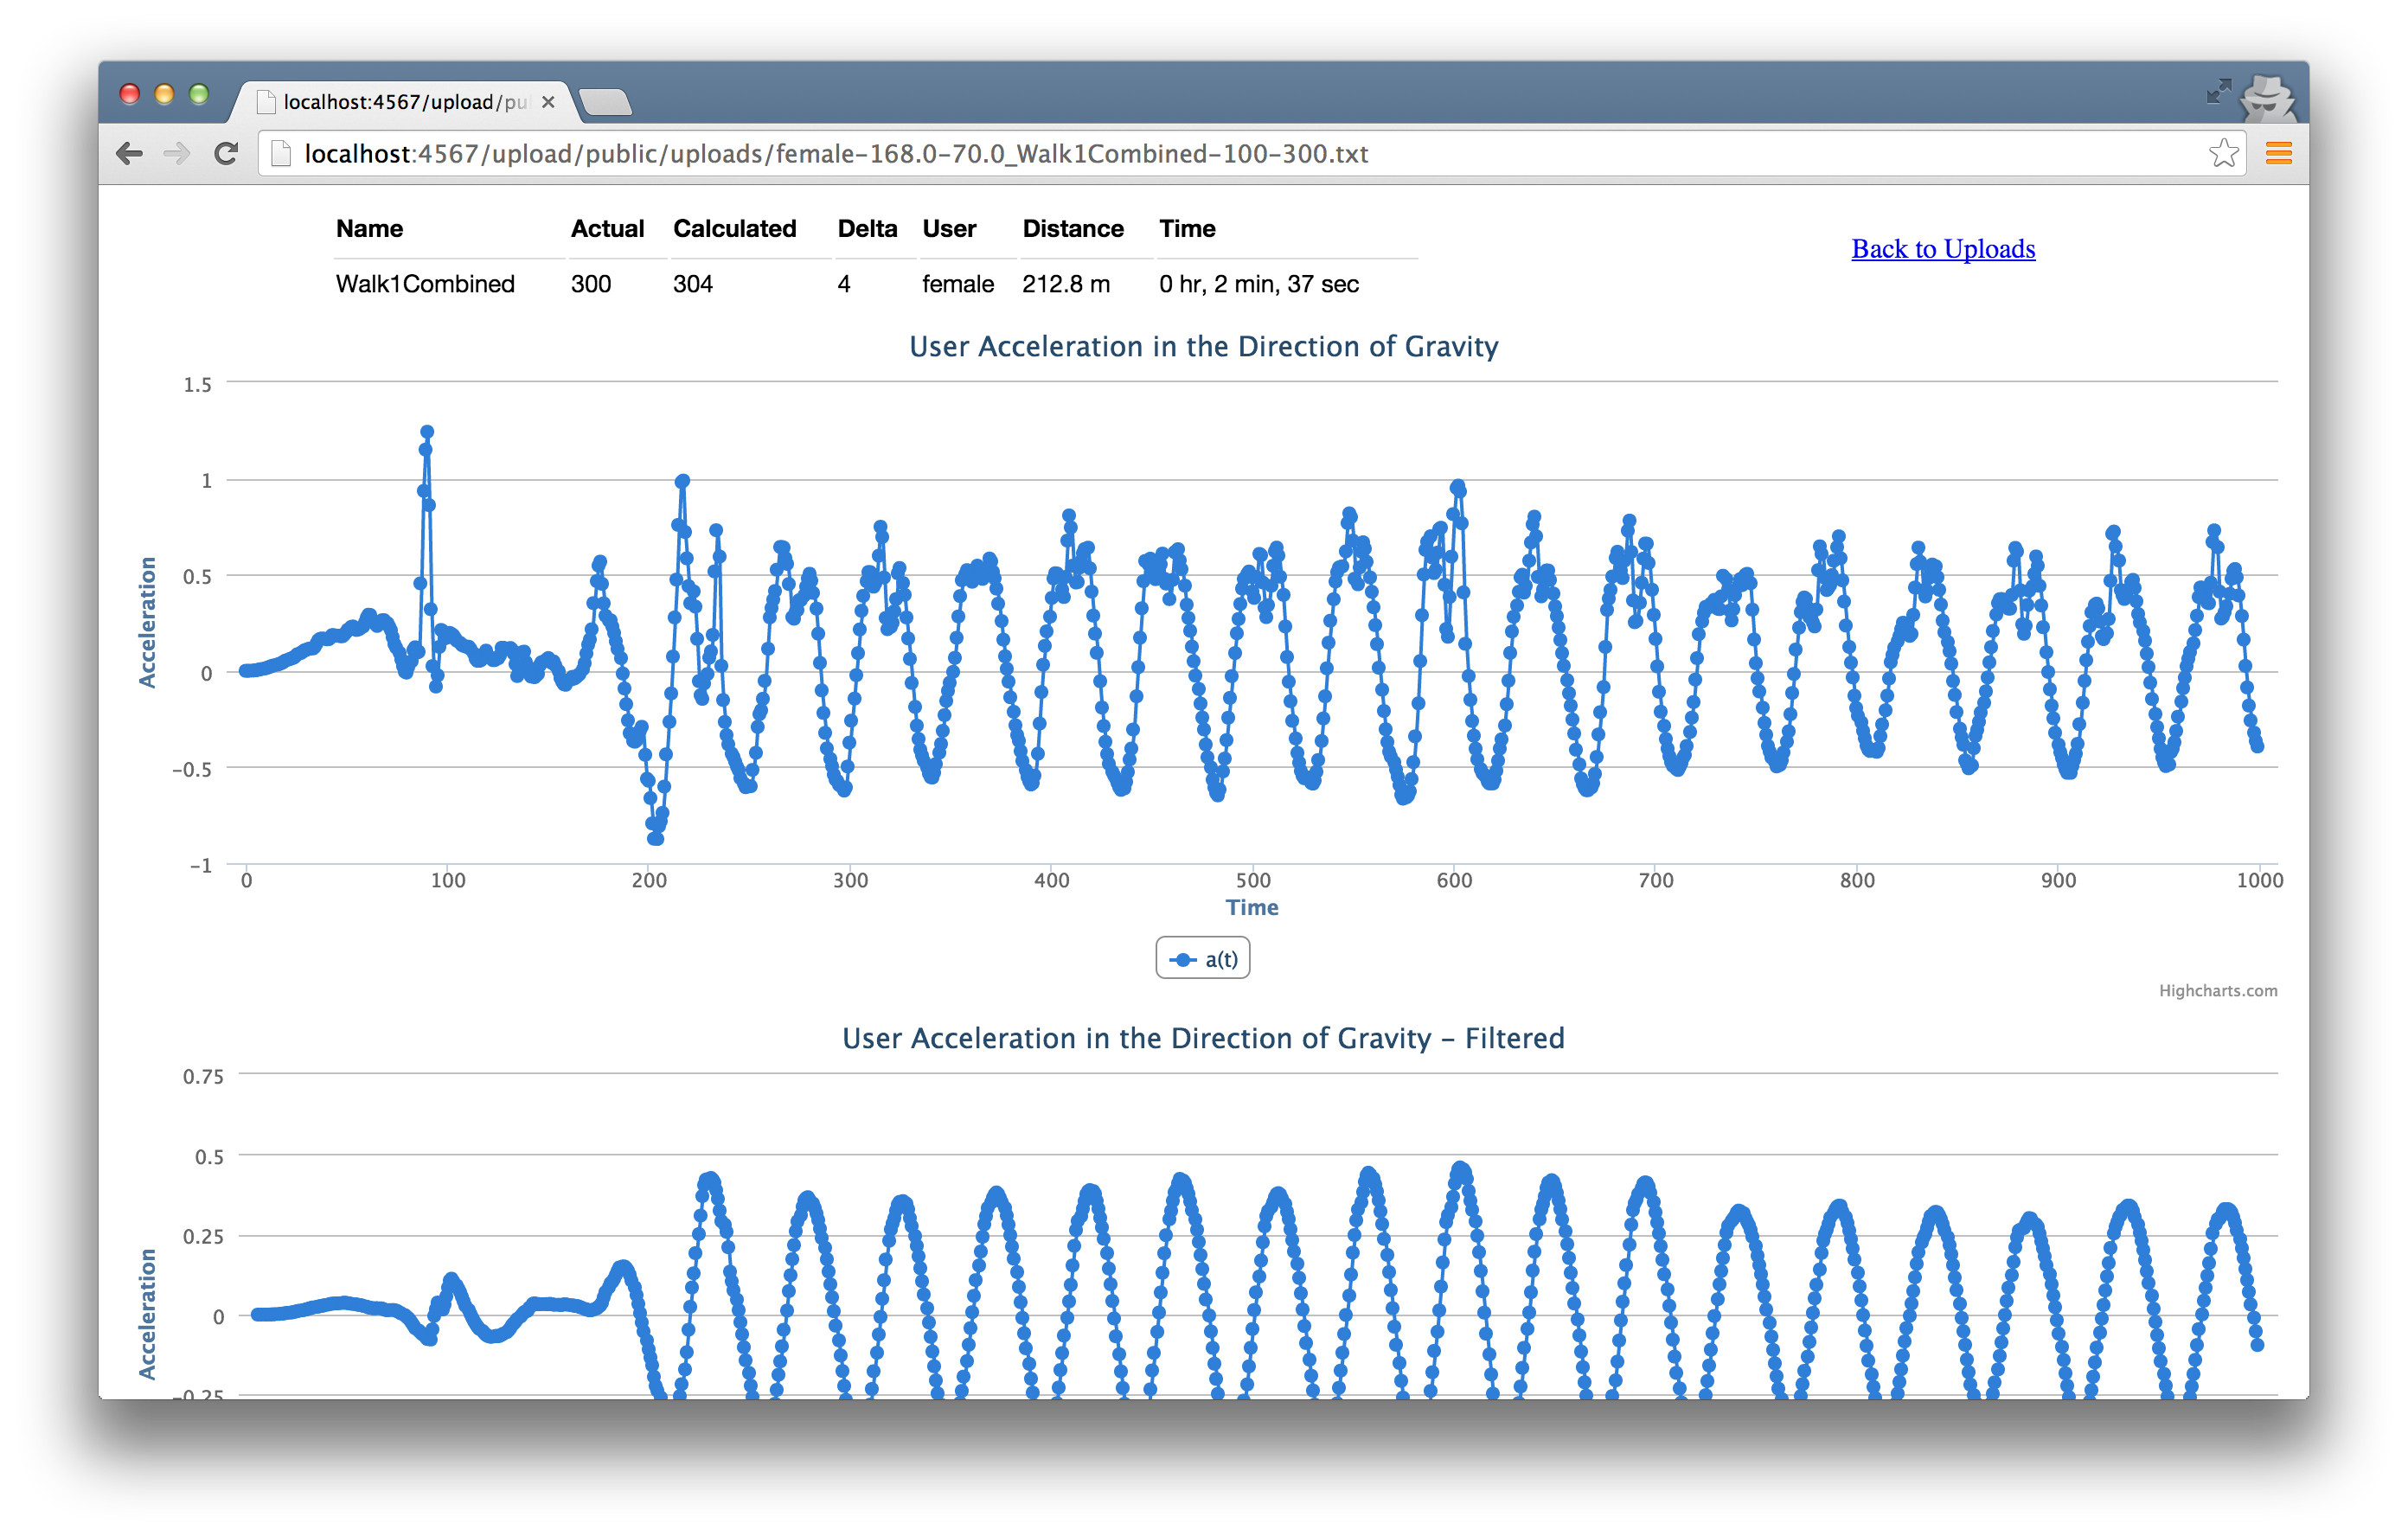
\includegraphics{chapter-figures/graffles/app3.png}\\ The information
presented includes values input by the user through the upload form,
values calculated by our program, and graphs of the time series
following the dot product operation, and again following filtering. The
user can navigate back to \texttt{/uploads} using the \emph{Back to
Uploads} link.

Let's look at what the outlined functionality above implies for us,
technically. We'll need two major components that we don't yet have:

\begin{aosaenumerate}
\def\labelenumi{\arabic{enumi}.}

\item
  A way to store and retrieve user input data.
\item
  A web application with a basic interface.
\end{aosaenumerate}

Let's examine each of these two requirements.

\aosasectii{1. Storing and Retrieving
Data}\label{storing-and-retrieving-data}

Our app needs to store input data to, and retrieve data from, the file
system. We'll create an \texttt{Upload} class to do this. Since the
class deals only with the file system and doesn't relate directly to the
implementation of the pedometer, we've left it out for brevity, but it's
worth discussing its basic functionality. Our \texttt{Upload} class has
three class-level methods for file system access and retrieval, all of
which return one or more instances of \texttt{Upload}:

\begin{aosaitemize}

\item
  \texttt{create} takes a file along with user and trial information. It
  stores the file to the file system, under a filename it generates to
  contain the user and trial information. The \texttt{@file\_path},
  \texttt{@user}, and \texttt{@trial} instance variables allow access to
  the file path, user object, and trial object, respectively.
\item
  \texttt{find} takes a file path and returns an instance of
  \texttt{Upload}.
\item
  \texttt{all} returns an array of \texttt{Upload} instances, one for
  each accelerometer data file in the file system.
\end{aosaitemize}

\aosasectiii{Separation of Concerns in
Upload}\label{separation-of-concerns-in-upload}

Once again, we've been wise to separate concerns in our program. All
code related to storage and retrieval is contained in the
\texttt{Upload} class. As our application grows, we'll likely want to
use a database rather than saving everything to the file system. When
the time comes for that, all we have to do it change the \texttt{Upload}
class. This makes our refactoring simple and clean.

In the future, we can save \texttt{User} and \texttt{Trial} objects to
the database. The \texttt{create}, \texttt{find}, and \texttt{all}
methods in \texttt{Upload} will then be relevant to \texttt{User} and
\texttt{Trial} as well. That means we'd likely refactor those out into
their own class to deal with data storage and retrieval in general, and
each of our \texttt{User}, \texttt{Trial}, and \texttt{Upload} classes
would inherit from that class. We might eventually add helper query
methods to that class, and continue building it up from there.

\aosasectii{2. Building a Web
Application}\label{building-a-web-application}

Web apps have been built many times over, so we'll leverage the
important work of the open source community and use an existing
framework to do the boring plumbing work for us. The Sinatra framework
does just that. In the tool's own words, Sinatra is ``a DSL for quickly
creating web applications in Ruby''. Perfect.

Our web app will need to respond to HTTP requests, so we'll need a file
that defines a route and associated code block for each combination of
HTTP method and URL. Let's call it \texttt{pedometer.rb}.

\begin{verbatim}
get '/uploads' do
  @error = "A #{params[:error]} error has occurred." if params[:error]
  @pipelines = Upload.all.inject([]) do |a, upload|
    a << Pipeline.run(File.read(upload.file_path), upload.user, upload.trial)
    a
  end

  erb :uploads
end

get '/upload/*' do |file_path|
  upload = Upload.find(file_path)
  @pipeline = Pipeline.run(File.read(file_path), upload.user, upload.trial)

  erb :upload
end

post '/create' do
  begin
    Upload.create(params[:data][:tempfile], params[:user], params[:trial])

    redirect '/uploads'
  rescue Exception => e
    redirect '/uploads?error=creation'
  end
end
\end{verbatim}

\texttt{pedometer.rb} allows our app to respond to HTTP requests for
each of our routes. Each route's code block either retrieves data from,
or stores data to, the file system through \texttt{Upload}, and then
renders a view or redirects. The instance variables instantiated will be
used directly in our views. The views simply display the data and aren't
the focus of our app, so we we'll leave the code for them out of this
chapter.

Let's look at each of the routes in \texttt{pedometer.rb} individually.

\aosasectiii{get \texttt{/uploads}}\label{get-uploads}

Navigating to \texttt{http://localhost:4567/uploads} sends an HTTP GET
request to our app, triggering our \texttt{get '/uploads'} code. The
code runs the pipeline for all of the uploads in the file system and
renders the \texttt{uploads} view, which displays a list of the uploads,
and a form to submit new uploads. If an error parameter is included, an
error string is created, and the \texttt{uploads} view will display the
error.

\aosasectiii{get \texttt{/upload/*}}\label{get-upload}

Clicking the \textbf{Detail} link for each upload sends an HTTP GET to
\texttt{/upload} with the file path for that upload. The pipeline runs,
and the \texttt{upload} view is rendered. The view displays the details
of the upload, including the charts, which are created using a
JavaScript library called HighCharts.

\aosasectiii{post \texttt{/create}}\label{post-create}

Our final route, an HTTP POST to \texttt{create}, is called when a user
submits the form in the \texttt{uploads} view. The code block creates a
new \texttt{Upload}, using the \texttt{params} hash to grab the values
input by the user through the form, and redirects back to
\texttt{/uploads}. If an error occurs in the creation process, the
redirect to \texttt{/uploads} includes an error parameter to let the
user know that something went wrong.

\aosasecti{A Fully Functional App}\label{a-fully-functional-app}

Voilà! We've built a fully functional app, with true applicability.

The real world presents us with intricate, complex challenges. Software
is uniquely capable of addressing these challenges at scale with minimal
resources. As software engineers, we have the power to create positive
change in our homes, our communities, and our world. Our training,
academic or otherwise, likely equipped us with the problem-solving
skills to write code that solves isolated, well-defined problems. As we
grow and hone our craft, it's up to us to extend that training to
address practical problems, tangled up with all of the messy realities
of our world. I hope that this chapter gave you a taste of breaking down
a real problem into small, addressable parts, and writing beautiful,
clean, extensible code to build a solution.

Here's to solving interesting problems in an endlessly exciting world.

\end{aosachapter}
